% **************************************************** <<< %
% DOCUMENT INFORMATION                                     %
% ******************************************************** %
%                                                          %
% Purpose of Document                                      %
% -------------------                                      %
% Defense of Thesis                                        %
%                                                          %
% Institution                                              %
% -----------                                              %
% University of Applied Sciences and Arts Northwestern     %
% Switzerland, School of Engineering                       %
%                                                          %
% Degree Program                                           %
% --------------                                           %
% Electrical and Information Technology, BSc.              %
%                                                          %
% Author & Copyright                                       %
% ------------------                                       %
% Raphael Frey, rmfrey@runbox.com                          %
% Noah Huesser, yatekii@yatekii.ch                         %
%                                                          %
% Date: 2017-SEP-15                                        %
% **************************************************** >>> %

% ================================================================= PREAMBLE <<<
% ----------------------------------------------------------- DOCUMENT CLASS <<<
\documentclass{beamer}                % Presentation Version
%\documentclass[trans]{beamer}         % Transparency Version
%\documentclass[handout]{beamer}       % Handout Version
%>>>
% ------------------------------------------------------------- Beamer Setup <<<
%\addtobeamertemplate{background canvas}{\transdissolve[duration=1]\hspace{-0.29em}}{}
%\usetheme[titleformat=smallcaps,numbering=none]{metropolis}
\usetheme[titleformat=smallcaps,progressbar=frametitle]{metropolis}
%>>>
% ----------------------------------------------------------------- Packages <<<
\usepackage[english]{babel}
\usepackage{xcolor-solarized}
\usepackage{lipsum}
\usetikzlibrary{calc}
\usetikzlibrary{positioning}
\usetikzlibrary{arrows}
\usetikzlibrary{calc}
\usetikzlibrary{fit}
\usetikzlibrary{backgrounds}
\usetikzlibrary{shapes.symbols}
\usepackage{dirtree}
\usepackage[outputdir=build,cachedir=mintedCache]{minted}
\usepackage{hologo}
\definecolor{da0}{HTML}{002B36}  \definecolor{da1}{HTML}{073642}
\definecolor{da2}{HTML}{008080}  \definecolor{da3}{HTML}{800080}
\definecolor{da4}{HTML}{404040}
\definecolor{br0}{HTML}{BEB9AA}  \definecolor{br1}{HTML}{EEE8D5}
\definecolor{br2}{HTML}{FDF6E3}
\definecolor{ct0}{HTML}{CB4B16}  \definecolor{ct1}{HTML}{DC322F}
\definecolor{ct2}{HTML}{DC3682}  \definecolor{ct3}{HTML}{268BD2}
\definecolor{ct4}{HTML}{2AA198}  \definecolor{ct5}{HTML}{B58900}
\definecolor{ct6}{HTML}{859900}  \definecolor{sq0}{HTML}{F7FBFF}
\definecolor{sq1}{HTML}{EFF3FF}  \definecolor{sq2}{HTML}{DECDF7}
\definecolor{sq3}{HTML}{C6DBEF}  \definecolor{sq4}{HTML}{BDD7E7}
\definecolor{sq5}{HTML}{9ECAE1}  \definecolor{sq6}{HTML}{6BAED6}
\definecolor{sq7}{HTML}{4292C6}  \definecolor{sq8}{HTML}{3182BD}
\definecolor{sq9}{HTML}{2171B5}  \definecolor{sqA}{HTML}{08519C}
\definecolor{sqB}{HTML}{084594}  \definecolor{sqC}{HTML}{08306B}
\definecolor{dv-7}{HTML}{8E0152} \definecolor{dv-6}{HTML}{C51B7D}
\definecolor{dv-5}{HTML}{D01C8B} \definecolor{dv-4}{HTML}{DE77AE}
\definecolor{dv-3}{HTML}{E9A3C9} \definecolor{dv-2}{HTML}{F1B6DA}
\definecolor{dv-1}{HTML}{FDE0EF} \definecolor{dv+0}{HTML}{F7F7F7}
\definecolor{dv+1}{HTML}{D1E5F0} \definecolor{dv+2}{HTML}{92C5DE}
\definecolor{dv+3}{HTML}{67A9CF} \definecolor{dv+4}{HTML}{4393C3}
\definecolor{dv+5}{HTML}{0571B0} \definecolor{dv+6}{HTML}{2166AC}
\definecolor{dv+7}{HTML}{053061}
\definecolor{q0}{named}{ct3}   \definecolor{q1}{named}{sqB}
\definecolor{q2}{named}{ct2}   \definecolor{q3}{named}{da3}
\definecolor{q4}{HTML}{FEC44F} \definecolor{q5}{named}{ct0}
\definecolor{q6}{HTML}{80EA82} \definecolor{q7}{HTML}{2E7D32}
\setminted{%
    %style=xcode,
    %style=trac,
    %style=paraiso-light,
    %style=lovelace,
    style=murphy,
    bgcolor=solarized-base3,
    linenos=false,
    autogobble,
}
\usepackage{booktabs}
\usepackage{pgfplots}
%\setbeamercolor{alerted text}{fg=solarized-red}
%>>>
% ------------------------------------------------------------------- Macros <<<
% Arrow for use in text
\def\tikzrarrow{%
    \tikz[baseline=-0.67ex]\draw[double,very thick,-{stealth}](0,0)--(0.5,0);}
\newlength{\yOffs}
\newlength{\xOffs}
\newcommand*\code[1]{\texttt{#1}}
\newcommand\source[1]{%
    \tikz[remember picture,overlay]
        \node[align=left,anchor=south west,text=solarized-base1,font=\tiny]
        at (current page.south west)
        {Quelle: #1};
}
% Node for use in Table/Text
\newcommand\contrastnode[1]{%
    \tikz[
        baseline=(n0.base),
        rounded corners=2mm,
        inner sep=5pt,
        text=solarized-base2,
    ]
        \node[fill=solarized-base01] (n0) {#1};
}
\newcommand*\XeLaTeX{\hologo{XeLaTeX}}
%>>>
% -------------------------------------------------------------- Title Setup <<<
\title{\vspace*{4em}\Large Front-End Signal Processing for Red Pitaya Spectrum Analyzer}
\subtitle{\hfill Bachelor Thesis}
\date{\today}
%\date{26. April 2017}
\author{%
    Raphael Frey%
    \hfill%
    \scriptsize\texttt{%
        \href{mailto:rmfrey@runbox.com}%
        {rmfrey@runbox.com}}\\[0.5mm]
    \small
    Noah H\"usser
    \hfill%
    \scriptsize\texttt{%
        \href{mailto:yatekii@yatekii.ch}%
        {yatekii@yatekii.ch}}}

%\institute{IME}
\titlegraphic{
\includegraphics[height=2em]{images/fhnwLogoDE-solarized-base02.eps}}
\subject{LaTeX -- Kurze Einf\"uhrung}
\keywords{LaTeX Introduction Primer FHNW Overview}
%http://web.fhnw.ch/cd/corporate-design/logos-fur-die-hochschulen
%>>>
%>>>
% **************************************************************************** %
\begin{document}
% **************************************************************************** %

\frame[plain]{\titlepage} % -------------------------------------- TITLE FRAME %


% ============================================================================ %
%
%                                 C H U N K S
%
% ============================================================================ %
% <<<
\section{Overview}

% ==============================================================================
%
%                 T H E O R E T I C A L   B A C K G R O U N D
%
% ==============================================================================
\chapter{Theoretical Background} % ------------------------------------------- %
\label{ch:theory}
% ---------------------------------------------------------------------------- %
% ==============================================================================
%
%                               O V E R V I E W
%
% ==============================================================================

This  chapter presents  a  brief  synopsis on  some  aspects  of digital  data
acquisition from  an analog source  and the processing  of that data,  and how
those issues pertain to our project. It  is not intended to be a comprehensive
treatise on the subject but shall serve  as a short refresher. At its end, the
reader should  have sufficient insight  to understand the basic  motivation of
our project from a theoretical point of view.

% ==============================================================================
%
%                              D S P   C H A I N
%
% ==============================================================================
\section{The Digital Signal Processing Chain}% <<< --------------------------- %
\label{sec:dsp_chain}
% ---------------------------------------------------------------------------- %

Digitally acquiring a signal generally requires at least the following steps:
\begin{itemize}\tightlist
        \item
            Passing the signal through an analog low-pass filter.
        \item
            Sampling and quantizing the filtered signal.
\end{itemize}

The   resulting   sequence  of   values   can   then  be   further   digitally
processed. The necessary  building blocks  for this  process are  portrayed in
Figure~\ref{fig:dspChain:blocks}.

\begin{figure}
    \centering
    \tikzsetnextfilename{dspChain}
\begin{tikzpicture}[
    dspBlock/.style={
        draw=sqC,
        rounded corners=1mm,
        fill=sq3,
        minimum height=3.5ex,
        minimum width=4em,
    },
    signalPath/.style={
        draw=q4,,
        fill=q4!50!white,
        circle,
        inner sep=0.3mm,
    }
]
    \coordinate (in) at (-1.5,0);
    \coordinate (out) at (7.5,0);

    \node[dspBlock] (LP)  at (0,0) {LP};
    \node[dspBlock] (ADC) at (3,0) {ADC};
    \node[dspBlock] (DSP) at (6,0) {DSP};

    \draw[-latex] (in)  -- (LP);
    \draw[-latex] (LP)  -- (ADC);
    \draw[-latex] (ADC) -- (DSP);
    \draw[-latex] (DSP) -- (out);

    \node[above      =1ex] (a1a) at (in)       {A};
    \node[above right=1ex] (a2a) at (LP.east)  {A};
    \node[above right=1ex] (d1a) at (ADC.east) {D};
    \node[above      =1ex] (d2a) at (out)      {D};

    \node[signalPath,below=4ex] (a1b) at (a1a) {\footnotesize 1};
    \node[signalPath,below=4ex] (a2b) at (a2a) {\footnotesize 2};
    \node[signalPath,below=4ex] (d1b) at (d1a) {\footnotesize 3};
\end{tikzpicture}

    \caption[The DSP Chain]{%
        The  basic  building   blocks  of  the  DSP  chain   from  its  analog
        input  to its  digitally processed  output.  From  left to  right: The
        analog  low-pass filter  (\emph{LP}), the  analog-to-digital converter
        (\emph{ADC}), and  an arbitrary  digital signal processing  system for
        further processing of the ADC's output (\emph{DSP}).%
    }
    \label{fig:dspChain:blocks}
\end{figure}

\begin{figure}
    \centering
    \tikzsetnextfilename{dspChainTimeDomain}
\begin{tikzpicture}[
    signalPath/.style={
        draw=q4,,
        fill=q4!50!white,
        circle,
        inner sep=0.3mm,
    }
]
     \pgfplotsset{every axis/.style={
            width=30mm,
            height=25mm,
            grid=none,
            axis line style={draw=none},
            tick style={draw=none},
            ticks = none,
        }
    }
    \begin{axis}[
        at = {(0,0)},
    ]
        \addplot[thick,q1,-] 
            table[x=t,y=y,col sep=comma] {images/dspChain/noisySine.csv};
    \end{axis}

    \begin{axis}[
        at = {(40mm,0)},
    ]
        \addplot[thick,q1,-,smooth] 
            table[x=t,y=y,col sep=comma] {images/dspChain/smoothSine.csv};
    \end{axis}

    \begin{axis}[
        at = {(80mm,0)},
    ]
        \addplot[q1,ycomb,mark=o,mark size=1.0]
            table[x=t,y=y,col sep=comma] {images/dspChain/sampledSine.csv};
    \end{axis}
    \draw[-latex] (2.9,1.25) -- (3.95,1.25);
    \draw[-latex] (6.9,1.25) -- (7.95,1.25);

    \node[signalPath] at (1.50,2.75) {\footnotesize 1};
    \node[signalPath] at (5.50,2.75) {\footnotesize 2};
    \node[signalPath] at (9.50,2.75) {\footnotesize 3};
\end{tikzpicture}

    \begin{tikzpicture}
     \pgfplotsset{every axis/.style={
            height=30mm,
            width=40mm,
            grid=none,
            axis line style={draw=none},
            tick style={draw=none},
            ticks = none,
        }
    }
    \begin{axis}[
        at = {(0,0)},
    ]
        \addplot[-] table[x=t,y=y,col sep=comma] {images/dspChain/spectrumFlat.csv};
    \end{axis}

    \begin{axis}[
        at = {(40mm,0)},
    ]
        \addplot[-,smooth] table[x=t,y=y,col sep=comma] {images/dspChain/spectrumLP.csv};
    \end{axis}

    \begin{axis}[
        at = {(80mm,0)},
    ]
        \addplot[-,smooth] table[x=t,y=y,col sep=comma] {images/dspChain/spectrumSampled.csv};
    \end{axis}
    \draw[-latex] (2.5,0.75) -- (3.85,0.75);
    \draw[-latex] (6.5,0.75) -- (7.85,0.75);

    \node[draw,inner sep=0.3mm,circle] at (1.25,1.75) {\footnotesize 1};
    \node[draw,inner sep=0.3mm,circle] at (5.25,1.75) {\footnotesize 2};
    \node[draw,inner sep=0.3mm,circle] at (9.25,1.75) {\footnotesize 3};
\end{tikzpicture}

    \caption[Signals Passing Through the DSP Chain (Simplified)]{%
        Simplified  time-domain  (top)   and  frequency-domain  (bottom)  view
        of  the  signal  at  different  stages on  its  way  through  the  DSP
        chain. The  circled  numbers  correspond  to the  stages  as  outlined
        in  Figure~\ref{fig:dspChain:blocks}.  Stage  1 is  the signal  before
        passing through the  input low-pass filter, with  a significant amount
        of  high-frequency noise. The  low-pass filter  removes any  frequency
        components  above ${f_s}/{2}$  in an  ideal scenario  (in reality,  it
        merely attenuates them, as we will see later), resulting in the signal
        at  stage  2.\protect\newline  After  having been  filtered,  the  ADC
        samples and  quantizes the signal,  yielding a sequence of  values, as
        schematically portrayed  in the rightmost  picture for stage  3.  Note
        that due to the sampling process,  the spectrum of the filtered signal
        is repeated at intervals of $f_s$. This  is the source of the issue of
        \emph{aliasing}.%
    }
    \label{fig:dspChain:signals}
\end{figure}

Of particular  interest for our  application is  what happens in  the ADC. The
quantization process converts a  value-continuous signal into a value-discreet
one,  with its  resolution being  a specification  of the  ADC which  is being
used. As an example, the ADC in our system has a resolution of \num{14}\,bits,
meaning it can divide its valid  input range into \num{16384} values. Given an
input  range of  \SI{2}{\volt_\mathrm{PP}}, this  equates to  a resolution  of
roughly \SI{122}{\micro\volt}  (in theory). This  quantization process  is the
source of what is generally known as \emph{quantization noise}.

Besides the quantization,  the other step happening in the  ADC is sampling; a
time-continuous signal is converted into a series of time-discreet values. The
time between those values is known as \emph{sampling time}, its inverse is the
\emph{sampling  frequency}. Note that  usually  these are  constant, at  least
during the  time where the signal  is measured. This need not  strictly be the
case  in theory  though. In our  system, this  sampling frequency  is a  fixed
property of the ADC, and is \SI{125}{\mega\hertz}.

The sampling  step lies  at the  core of  the problem  our project  intends to
address:  \emph{aliasing}. Therefore, we  will take  a  closer look  at a  few
consequences  of the  sampling  process, and  how they  are  relevant to  this
project.

Descriptively, the sampling  process can be thought of as  looking at a signal
at  specific points  in  time and  capturing  its value. Mathematically,  this
amounts to multiplying  the signal with a  series of Dirac pulses  in the time
domain,  and  convolving with  a  series  of  Dirac  pulses in  the  frequency
domain\footnotemark.
\footnotetext{%
    \emph{Pro memoria}: A series of Dirac pulses  in the time domain has as its
    spectrum a series of Dirac pulses as well.%
}.
This  convolution  in   the  frequency  domain  lies  at  the   heart  of  the
problem   of  aliasing,   because  it   results  in   the  incoming   signal's
spectrum  being  repeated  at  intervals  of  $f_s$  (see  also:  stage  3  in
Figure~\ref{fig:dspChain:signals}). This is no problem as long as the spectrum
of the incoming signal fits within  the boundaries set by this repetition. But
if  the  spectrum   of  the  incoming  signal  is  too   broad,  two  or  more
recurrences  of  the spectrum  will  overlap. This  effect is  highlighted  in
Figure~\ref{fig:aliasing:band}.

\begin{figure}
    \centering
    \begin{tikzpicture}
     \pgfplotsset{every axis/.style={
            height=40mm,
            width=120mm,
            grid=none,
            axis x line=bottom,
            axis y line=middle,
            xtick={-400,-200,0,200,400},
            xticklabel style={font=\footnotesize},
            xticklabels={
                $-f_s$,
                $-\frac{f_s}{2}$,
                $0$,
                $\frac{f_s}{2}$,
                $f_s$,
            },
            yticklabels={},
            ytick style={draw=none},
            xlabel={$f$},
            xlabel style={
                at={(ticklabel* cs:1.05)},
                anchor=east,
            },
            ymin=0,
            ymax=1,
        }
    }
    \begin{axis}[
        at = {(0mm,35mm)},
            xmin=-800,
            xmax=800,
            ymin=0,
            ymax=1.1,
    ]
        \addplot[smooth,-] table[x=f,y=Y,col sep=comma] {images/aliasing/bandNoAliasing.csv};
        \addplot[ycomb,mark=none,gray,style={dotted,thick}] coordinates {
            (-400,1.1)
            (-200,1.1)
            ( 200,1.1)
            ( 400,1.1)
        };
        \addplot[ycomb,mark=none,gray,style={dotted,thick}] coordinates {
            (-400,1.1)
            (-200,1.1)
            ( 200,1.1)
            ( 400,1.1)
        };
    \end{axis}

    \begin{axis}[
        at = {(0mm,0mm)},
        xmin=-800,
        xmax=+800,
        ymin=0,
        ymax=1.1,
    ]
        \addplot[name path=zero,black,very thin] coordinates {
            (-800,0) 
             (800,0)
        };

        \addplot[smooth,       -] table[x=f,y=Y,col sep=comma] {images/aliasing/bandAliased1.csv};
        \addplot[smooth,name path=uno,-] table[x=f,y=Y,col sep=comma] {images/aliasing/bandOverlap1.csv};
        \addplot[smooth,       -] table[x=f,y=Y,col sep=comma] {images/aliasing/bandAliased2.csv};
        \addplot[smooth,name path=due,-] table[x=f,y=Y,col sep=comma] {images/aliasing/bandOverlap2.csv};
        \addplot[smooth,       -]            table[x=f,y=Y,col sep=comma] {images/aliasing/bandAliased3.csv};

        \addplot[q2] fill between[
            of = uno and zero,
        ];
        \addplot[q2] fill between[
            of = due and zero,
        ];
        \addplot[ycomb,mark=none,gray,style={dotted,thick}] coordinates {
            (-400,1.1)
            (-200,1.1)
            ( 200,1.1)
            ( 400,1.1)
        };
    \end{axis}
\end{tikzpicture}

    \caption[Aliasing Illustrated via Signal Frequency Band]{%
        Simplified view  of a signal  which does not produce  aliasing between
        its recurrences  in the  frequency spectrum  (top), contrasted  with a
        signal whose  frequency band  has components  above half  the sampling
        frequency,  resulting   in  aliasing;  its  spectral   copies  overlap
        (highlighted areas in the bottom plot).%
    }
    \label{fig:aliasing:band}
\end{figure}

This overlap results in two primary problems:
\begin{itemize}\tightlist
    \item
        The digital  signal may not  be unambiguously reconstructable  into an
        analog signal, if that is intended.
    \item
        Frequencies  may occur  in the  digital  signal stream  which are  not
        actually  present  in  the  original  signal. This  problem  is  often
        referred to  as the  \emph{folding back} of  frequency components. See
        Figure~\ref{fig:aliasing:dirac} for an illustration  of how this might
        look.

        This problem is of particular interest  to our application, as we will
        see later.
\end{itemize}

\begin{figure}
    \centering
    \tikzsetnextfilename{aliasingDirac}
\begin{tikzpicture}
     \pgfplotsset{every axis/.style={
            height=30mm,
            width=\textwidth,
            grid=none,
            axis x line=bottom,
            axis y line=middle,
            %axis line style={draw=none},
            %tick style={draw=none},
            %ticks = none,
            yticklabels={},
            ytick style={draw=none},
            ymin=0,
            ymax=1.33,
            xlabel={$f$},
            xlabel style={
                at={(ticklabel* cs:1.05)},
                anchor=east,
            },
            xmin=-8,
            xmax=8,
            ylabel={$\delta(f)$},
            legend columns=3,
        },
        every axis legend/.append style={
            %at={(1.05,1.1)}, % if attached to top plot
            at={(0.5,2.6)},  % if attached to bottom plot
            anchor=south,
            font=\footnotesize,
            cells={anchor=east},
        },
    }
    % fs = 4
    % fs/2 = 2
    
    % Dirac at f=1
    \begin{axis}[
        at = {(0,0)},
        xtick={-6,-4,-2,-1,0,1,2,4,6},
        xticklabels={
            $-\frac{3f_s}{2}$,
            $-f_s$,
            $-\frac{f_s}{2}$,
            \raisebox{-6ex}{$-f_{\mathrm{sig}}$},
            0,
            \raisebox{-6ex}{$f_{\mathrm{sig}}$},
            $\frac{f_s}{2}$,
            $f_s$,
            $\frac{3f_s}{2}$},
        xticklabel style={font=\footnotesize},
    ]
        % Centered around 0
        \addplot[q3,thick,ycomb,mark=triangle*,mark options={scale=2.0}] coordinates {
            (1,1)
            (-1,1)
        };
        % Centered around fs = 4
        \addplot[thick,q1,ycomb,mark=triangle*,mark options={scale=2.0}] coordinates {
            (3,1)
            (5,1)
        };
        % Centered around -fs = -4
        \addplot[thick,q5,ycomb,mark=triangle*,mark options={scale=2.0}] coordinates {
            (-3,1)
            (-5,1)
        };

        % Centered around +-2fs = +-8
        \addplot[thick,br0,ycomb,mark=triangle*,mark options={scale=2.0}] coordinates {
            (7,1)
        };
        \addplot[thick,br1,ycomb,mark=triangle*,mark options={scale=2.0}] coordinates {
            (-7,1)
        };

        % Sampling Frequency and its half
        \addplot[thick,gray,ycomb,mark=none,style={dashed,thick}] coordinates {
            (2,0.75)
            (-2,0.75)
            (6,0.75)
            (-6,0.75)
        };
        \addplot[thick,gray,ycomb,mark=none,style={dashed,thick}] coordinates {
            (4,1.33)
            (-4,1.33)
        };
    \end{axis}

    % Dirac at f=3
    \begin{axis}[
        at = {(0mm,-43mm)},
        xtick={-6,-4,-3,-2,0,2,3,4,6},
        xticklabels={
            $-\frac{3f_s}{2}$,
            $-f_s$,
            \raisebox{-6ex}{$-f_{\mathrm{sig}}$},
            $-\frac{f_s}{2}$,
            0,
            $\frac{f_s}{2}$,
            \raisebox{-6ex}{$f_{\mathrm{sig}}$},
            $f_s$,
            $\frac{3f_s}{2}$},
        xticklabel style={font=\footnotesize},
    ]
        % Centered around 0
        \addplot[thick,q3,ycomb,mark=triangle*,mark options={scale=2}] coordinates {
            (3,1)
            (-3,1)
        };
        \addlegendentry{copy centered around $f=0$}

        % Centered around fs = 4
        \addplot[thick,q1,ycomb,mark=triangle*,mark options={scale=2}] coordinates {
            (1,1)
            (7,1)
        };
        \addlegendentry{copy centered around $f=f_s$}
        % Centered around -fs = -4
        \addplot[thick,q5,ycomb,mark=triangle*,mark options={scale=2}] coordinates {
            (-1,1)
            (-7,1)
        };
        \addlegendentry{copy centered around $f=-f_s$}

        % Centered around +-2fs = +-8
        \addplot[thick,br0,ycomb,mark=triangle*,mark options={scale=2}] coordinates {
            (5,1)
        };
        \addlegendentry{copy centered around $f=2f_s$}
        \addplot[thick,br1,ycomb,mark=triangle*,mark options={scale=2}] coordinates {
            (-5,1)
        };
        \addlegendentry{copy centered around $f=-2f_s$}

        % Sampling Frequency and its half
        \addplot[thick,gray,ycomb,mark=none,style={dashed,thick}] coordinates {
            (2,0.75)
            (-2,0.75)
            (6,0.75)
            (-6,0.75)
        };
        \addplot[thick,gray,ycomb,mark=none,style={dashed,thick}] coordinates {
            (4,1.33)
            (-4,1.33)
        };
    \end{axis}
\end{tikzpicture}

    \caption[Aliasing With Harmonic Signals]{%
        Example of  two harmonic signals  being sampled. In the top  plot, the
        signal's frequency is  below half the sampling frequency  and there is
        no aliasing. The  signal can be  reconstructed without error.   In the
        bottom  plot,  the  signal's  frequency is  above  half  the  sampling
        frequency. Consequently, the copies of the signal's frequency spectrum
        centered around  the sampling  frequency and  its negative  alias back
        into  the  band  between  $-f_s/2$  and  $f_s/2$. If  this  signal  is
        reconstructed, the resulting  signal would have a frequency  of $f_s -
        f_{\mathrm{sig}}$ instead of $f_{\mathrm{sig}}$.%
    }
    \label{fig:aliasing:dirac}
\end{figure}


Once a signal  has left the ADC and  is handed down the DSP  chain for further
processing,  the primary  problem becomes  one of  resources, particularly  in
real-time applications. In  most systems,  the available  hardware is  a fixed
constraint, and depending on what sort of processing is to be conducted on the
digital data stream, the available resources may or may not suffice.

If available resources are found to be insufficient for real-time processing of
the data stream, one may choose to
\begin{itemize}\tightlist
    \item
        not process the data in real time,
    \item
        reduce the complexity of the computations, or
    \item
        reduce the amount of data to be processed through \emph{downsampling}
        of the signal.
\end{itemize}
The  last case  is the  route  which is  chosen in  our application. The  main
constraint on the Red Pitaya is that  the data being generated cannot be moved
off the device in  real time, and the device itself  does not offer sufficient
storage for capturing a meaningful amount of data which can then be moved onto
another device for  further processing at a later  point. Therefore the amount
of data must  be reduced before it can  be moved off the device  to a computer
for viewing or further processing (see Section~\ref{sec:requirements}).

Because downsampling a signal is in  essence nothing more than the sampling of
a signal which has already been sampled, a lot of the considerations which are
valid for the  step from an analog  to a digital signal as  outlined above are
either very  similar or even identical. Specifically,  the same considerations
for  aliasing still  apply: If  the  signal which  is  to  be downsampled  has
frequency components  above $f_{s,  downsampled}/2$, aliasing  will occur. And
since  the signal  coming out  of  the ADC  has the  analog signal's  spectrum
(filtered by the analog lowpass before  the ADC) recurring at intervals of the
ADC's sampling frequency, this is always the case.

Therefore,  the sampled  signal must  be  filtered through  a low-pass  filter
before  being downsampled,  just as  the original  analog signal  was low-pass
filtered  before being  passed into  the  ADC. In light  of the  signal to  be
downsampled  being a  \emph{digital} signal  instead  of an  analog one,  that
low-pass filter must  naturally be a digital filter as  well. Designing such a
digital low-pass filter is the core mission of this project.

The key properties of such a filter which are relevant to our application are
\begin{itemize}\tightlist
    \item
        its transition band width (filter steepness), and
    \item
        its aliasing attenuation.
\end{itemize}
The aliasing attenuation refers  to the fact that when a  filter is being used
for  downsampling,  copies  of  its  frequency response  will  be  created  at
intervals  of the  lower  sampling  rate (analogous  to  the sampling  process
producing spectral copies of a signal when sampling an analog signal).

The stopband  components of these  copies overlap with the  intended passband,
leading to aliasing  (it should be noted that this  phenomenon is also present
in the  case of  the analog input  filter for the  DSP chain). This  effect is
portrayed  in  Figure~\ref{fig:aliasing:iirCopies}. The  top  plot  shows  the
filter's frequency response  along with four copies to  illustrate the overlap
effect. The bottom plot shows the aliasing effect more clearly by removing the
spectral copies and retaining the aliased regions.

The overlapping parts of the spectrum  are composed of spectral copies both to
the right  and left side of  the original. Therefore, the aliased  regions are
alternately flipped around the vertical axis. This creates in essence the same
effect  as if  the paper  were folded  along multiples  of the  lower sampling
rate  over the  frequency  range of  the  central  copy (in  the  case of  our
example: $0.2f_s$, $0.4f_s$, $0.6f_s$ and $0.8f_s$) like an accordion. This is
where the term \emph{folding back} originates.

\begin{figure}
    \centering
    %\tikzsetnextfilename{iirCopies}
\newcommand*\freqzFileCICA{images/iirCopies/iirAliasingZero.csv}
\newcommand*\freqzFileCICB{images/iirCopies/iirAliasingP2.csv}
\newcommand*\freqzFileCICC{images/iirCopies/iirAliasingN2.csv}
\newcommand*\freqzFileCICD{images/iirCopies/iirAliasingP4.csv}
\newcommand*\freqzFileCICE{images/iirCopies/iirAliasingN4.csv}
\newcommand*\freqzFileCICF{images/iirCopies/iirAliasingCleanZero.csv}
\newcommand*\freqzFileCICG{images/iirCopies/iirAliasingCleanP2.csv}
\newcommand*\freqzFileCICH{images/iirCopies/iirAliasingCleanN2.csv}
\newcommand*\freqzFileCICI{images/iirCopies/iirAliasingCleanP4.csv}
\newcommand*\freqzFileCICJ{images/iirCopies/iirAliasingCleanN4.csv}
\pgfplotstableread[col sep=comma]{\freqzFileCICA}\freqzTableCICA
\pgfplotstableread[col sep=comma]{\freqzFileCICB}\freqzTableCICB
\pgfplotstableread[col sep=comma]{\freqzFileCICC}\freqzTableCICC
\pgfplotstableread[col sep=comma]{\freqzFileCICD}\freqzTableCICD
\pgfplotstableread[col sep=comma]{\freqzFileCICE}\freqzTableCICE
\pgfplotstableread[col sep=comma]{\freqzFileCICF}\freqzTableCICF
\pgfplotstableread[col sep=comma]{\freqzFileCICG}\freqzTableCICG
\pgfplotstableread[col sep=comma]{\freqzFileCICH}\freqzTableCICH
\pgfplotstableread[col sep=comma]{\freqzFileCICI}\freqzTableCICI
\pgfplotstableread[col sep=comma]{\freqzFileCICJ}\freqzTableCICJ
\begin{tikzpicture}[
%    trim axis left,
%    trim axis right,
]
     \pgfplotsset{every axis/.style={
            width=\textwidth,
            grid=none,
            y filter/.code={\pgfmathparse{20*log10(\pgfmathresult))}},
            x filter/.code={\pgfmathparse{\pgfmathresult / 3.141592654}},
            xlabel=Normalized Frequency,
            ylabel=Magnitude,
            x unit=\times\,\pi\,\si{\radian}/\si{\sample},
            y unit=\si{dB},
        },
    }
    \begin{axis}[
            %title={Folding Back Due to Spectral Copies{,} $f_\mathrm{s,low} = \frac{f_\mathrm{s,high}}{5}$},
            at = {(0,0)},
            height=50mm,
            xmin=-1.8,
            xmax=1.8,
            ymin=-120,
            ymax=5,
            xtick={
                -1,
                %-0.8,
                %-0.4,
                0,
                %0.4,
                %0.8,
                1%
            },
            xticklabels={%
                $-f_\mathrm{s,high}/2$,
                %$-2 \cdot f_\mathrm{s,low}$,
                %$-1 \cdot f_\mathrm{s,low}$,
                $0$,
                %$1 \cdot f_\mathrm{s,low}$,
                %$2 \cdot f_\mathrm{s,low}$,
                $f_\mathrm{s,high}/2$%
            },
            %xticklabel style={rotate=90},
        ]
        \fill[q2!20!white] (0.2,5) rectangle (0.4,-120);
        \fill[q0!20!white] (0.4,5) rectangle (0.6,-120);
        \fill[q5!20!white] (0.6,5) rectangle (0.8,-120);
        \fill[q7!20!white] (0.8,5) rectangle (1.0,-120);

        \draw[black] (0,5) -- (0,-120);

        \addplot[q2,-]            table[x=w, y=abs(H)] \freqzTableCICB;
        \addplot[q0,-]            table[x=w, y=abs(H)] \freqzTableCICC;
        \addplot[q5,-]            table[x=w, y=abs(H)] \freqzTableCICD;
        \addplot[q7,-]            table[x=w, y=abs(H)] \freqzTableCICE;
        \addplot[very thick,q1,-] table[x=w, y=abs(H)] \freqzTableCICA;

        % The rectangles draw over the axis lines
        \draw (0.2,   5) -- (1,   5);
        \draw (0.2,-120) -- (1,-120);
    \end{axis}

    %\begin{axis}[
    %        title={Folding Back Due to Spectral Copies: Detail},
    %        at = {(0,-125mm)},
    %        height=90mm,
    %        xmin=0,
    %        xmax=1,
    %        ymin=-120,
    %        ymax=5,
    %        xtick={
    %            0,
    %            0.2,
    %            0.4,
    %            0.6,
    %            0.8,
    %            1%
    %        },
    %        xticklabels={%
    %            $0$,
    %            $1 \cdot f_\mathrm{s,low}$,
    %            $2 \cdot f_\mathrm{s,low}$,
    %            $3 \cdot f_\mathrm{s,low}$,
    %            $4 \cdot f_\mathrm{s,low}$,
    %            $f_\mathrm{s,high}/2$%
    %        },
    %        xticklabel style={rotate=90},
    %    ]
    %    \fill[q2!20!white] (0.2,5) rectangle (0.4,-120);
    %    \fill[q0!20!white] (0.4,5) rectangle (0.6,-120);
    %    \fill[q5!20!white] (0.6,5) rectangle (0.8,-120);
    %    \fill[q7!20!white] (0.8,5) rectangle (1.0,-120);

    %    \addplot[thick,q2,-] table[x=w, y=abs(H)] \freqzTableCICG;
    %    \addplot[thick,q0,-] table[x=w, y=abs(H)] \freqzTableCICH;
    %    \addplot[thick,q5,-] table[x=w, y=abs(H)] \freqzTableCICI;
    %    \addplot[thick,q7,-] table[x=w, y=abs(H)] \freqzTableCICJ;
    %    \addplot[very thick,q1,-] table[x=w, y=abs(H)] \freqzTableCICF;

    %    % The rectangles draw over the axis lines
    %    \draw (0.2,   5) -- (1,   5);
    %    \draw (0.2,-120) -- (1,-120);
    %    \draw (1,     5) -- (1,-120);
    %\end{axis}
\end{tikzpicture}

    \caption[Folding Back of Stopband Components Into Passband]{%
        The phenomenon  of folding back  when downsampling, illustrated  for a
        lowpass IIR  filter with a  cutoff frequency  of $0.2\cdot f_s$  for a
        downsampling ratio of $R=5$.  The downsampling process produces copies
        of the filter's frequency response  at intervals of the lower sampling
        frequency, visible  in the  top plot.  The  stopbands of  these copies
        then  overlap with  the intended  passband.  The  bottom plot  shows a
        close-up view with the spectral copies for clarity.%
    }
    \label{fig:aliasing:iirCopies}
\end{figure}

%>>>
% ==============================================================================
%
%                        D I G I T A L   F I L T E R S
%
% ==============================================================================
\section{Digital Filters}% <<< ----------------------------------------------- %
\label{sec:digital_filters}
% ---------------------------------------------------------------------------- %

Digital filters can  be distinguished by several  characteristics; common ways
to  categorize them  are by  topology,  impulse response  and their  frequency
response. There  are  two commonly  used  types  of digital  filters: Infinite
impulse   response   (IIR)  filters   and   finite   impulse  response   (FIR)
filters. Another important class of filters are cascaded integrator-comb (CIC)
filters,  however, in  the strictest  sense they  are a  special class  of FIR
filters rather than an entirely new  type of LTI system~\cite{1163535}.  While
our system uses FIR and CIC filters,  a brief overview of IIR filters is still
presented here, for the sake of completeness.
% ==============================================================================
%
%                        I I R   F I L T E R S
%
% ==============================================================================
\subsection{IIR Filters} %<<< ------------------------------------------------ %
\label{subsec:iir_filters}
% ---------------------------------------------------------------------------- %

Infinite impulse response filters are  so named because their impulse response
continues  into perpetuity,  never  reaching zero. In  practice, the  response
usually comes  sufficiently close to  zero at a certain  point that it  can be
considered zero for most intents and purposes.

IIR filters have feedback paths, resulting  in a filter response equation with
non-trivial  denominator components. Their  basic  building  blocks are  delay
elements, multipliers and adders.

\begin{equation}
    \label{eq:iir_filter}
    H(z) = \frac{%
            \sum_{k=0}^N b_k \cdot z^{-k}}{%
            1 + \sum_{i=0}^M a_i \cdot z^{-i}}
\end{equation}

IIR filters generally require a lower order (and therefore fewer resources) to
approximate a  certain frequency  response specification  than FIR  filters do
(particularly the constraint of a narrow transition band), but this comes at a
cost:  IIR  filters have a  non-linear phase response;  linear-phase responses
can only  be approximated. Furthermore, IIR  filters are not guaranteed  to be
BIBO stable due to their feedback paths.

\begin{figure}
    \centering
    % https://tex.stackexchange.com/a/183092/131649
\begin{tikzpicture}[
    triangle/.style = {draw,regular polygon, regular polygon sides=3 },
    node rotated/.style   = {rotate=180},
    border rotatedA/.style = {shape border rotate=-90},
    border rotatedB/.style = {shape border rotate=90},
]    
    \coordinate (in)  at (0,0);
    \coordinate (out) at (8,0);

    % Delay elements
    \node[draw] (d1) at  (2,-1) {$z^{-1}$};
    \node[draw] (d2) at  (2,-3) {$z^{-1}$};
    \node[draw] (d3) at  (6,-1) {$z^{-1}$};
    \node[draw] (d4) at  (6,-3) {$z^{-1}$};

    % Multipliers
    \node[triangle, border rotatedA] (m1) at  (3,0) {};
    \node[triangle, border rotatedA] (m2) at  (3,-2) {};
    \node[triangle, border rotatedA] (m3) at  (3,-4) {};
    \node[triangle, border rotatedA] (m4) at  (5,0) {};
    \node[triangle, border rotatedB] (m5) at  (5,-2) {};
    \node[triangle, border rotatedB] (m6) at  (5,-4) {};

    %% Adders
    \node[draw,circle, inner sep=0.3mm] (a1) at  (4,0) {$+$};
    \node[draw,circle, inner sep=0.3mm] (a2) at  (4,-2) {$+$};
    \node[draw,circle, inner sep=0.3mm] (a3) at  (4,-4) {$+$};

    %% Lines
    \draw[-latex] (in) -- (m1);
    \draw[-latex] (in) -| (d1);
    \draw[-latex] (d1) -- (d2);
    \draw[-latex] (d1) |- (m2);
    \draw[-latex] (d2) |- (m3);
    \draw[-latex] (m1) -- (a1);
    \draw[-latex] (m2) -- (a2);
    \draw[-latex] (m3) -- (a3);
    \draw[-latex] (a1) -- (m4);
    \draw[-latex] (m5) -- (a2);
    \draw[-latex] (m6) -- (a3);
    \draw[-latex] (d3) |- (m5);
    \draw[-latex] (d3) -- (d4);
    \draw[-latex] (d4) |- (m6);
    \draw[-latex] (m4) -| (d3);
    \draw[-latex] (m4) -- (out);
\end{tikzpicture}

    \caption[IIR Filter: Biquad]{Example of an IIR filter topology for a biquad}
    \label{fig:filtertopologies:iir}
\end{figure}

Some of the generally used types of IIR filters are:
\begin{itemize}\tightlist
    \item
        Butterworth  filter: Named after  the British  engineer and  physicist
        Stephen  Butterworth  (1885  --  1958),  who  first  described  it  in
        1930. Characterized by a very flat passband (no passband ripple).
    \item
        Chebyshev filter  (type I  and II): Named after  Russian mathematician
        Pafnuty Chebyshev  (1821 --  1894). They are steeper  than Butterworth
        filters, at the cost of suffering from ripple in the passband (type I)
        or stopband (type II).
    \item
        Bessel  filter: Named for  the German  mathematician Friedrich  Bessel
        (1784 -- 1846). Optimized to have a maximally linear phase response in
        order  to  minimize the  distortion  of  signals passing  through  the
        filter.
    \item
        Elliptical  filters: Also known  as  Cauer filters,  after the  German
        mathematician Wilhelm Cauer (1900 -- 1945), or Zolotarev filter, after
        Russian mathematician Yegor Zolotarev (1847 -- 1878). Characterized by
        equiripple in the  bassband and stopband and a  very narrow transition
        band compared to other filters of the same order.
\end{itemize}
Digital IIR filters are often designed by way of the bilinear transform.

%>>>
% ==============================================================================
%
%                            F I R   F I L T E R S
%
% ==============================================================================
\subsection{FIR Filters} %<<< ------------------------------------------------ %
\label{subsec:FIR_filters}
% ---------------------------------------------------------------------------- %

FIR filters are  characterized by an impulse response which  decays to zero in
finite time (see  Figure~\ref{fig:filter_specs:coefs}, unlike IIR filters. The
filter response is characterized by Equation~\ref{eq:fir_filter}:

\begin{equation}
    \label{eq:fir_filter}
    H(z) = \sum_{k=0}^{N} b_k \cdot z^{-k}
\end{equation}

FIR filters have several advantages:

\begin{itemize}\tightlist
    \item
        They are inherently BIBO stable because they lack feedback paths.
    \item
        They  can  be  easily  designed  to  have  a  linear  phase  response,
        preventing signal distortion due to  different group delays for signal
        components of different frequencies.
    \item
        The shape of  their frequency response can be  very finely tuned. This
        makes them ideally  suited for certain purposes,  such as compensation
        filters (see Section~\ref{subsec:CIC_filters}).
    \item
        Implementation is usually rather straightforward.
\end{itemize}

Their  main  disadvantage   is  that  due  to  the  lack   of  feedback,  they
generally require comparatively high filter  orders for narrow transition band
widths. Illustratively, this can be understood by the following considerations:
\begin{itemize}\tightlist
    \item
        The frequency response of an ideal low-pass filter is the brick wall
        filter, i.e. a rectangle.
    \item
        The inverse  Fourier transform  of a rectangle  is a  $sinc$ function,
        which is infinitely long.
    \item
        Therefore, the impulse  response of the ideal brick  wall filter would
        have an infinite number of taps.
    \item
        Truncation of the number of taps  leads to a deviation of the filter's
        frequency response from the brick wall  filter.  As the number of taps
        (and  therefore the  FIR filter's  impulse response)  is reduced,  its
        frequency response deviates more and  more from the brick wall filter,
        resulting  in  a  flatter  transition between  the  passband  and  the
        stopband as well as the introduction of ripple.
\end{itemize}

This     process     is     illustrated      in     simplified     form     in
Figure~\ref{fig:brick_wall_vs_FIR}.

The  FIR filter's  transition band  width  is particularly  important for  our
application in order to reduce aliasing effects, as will be shown later.

\begin{figure}
    \centering
    \begin{tikzpicture}
     \pgfplotsset{every axis/.style={
            height=40mm,
            width=60mm,
            grid=none,
            axis x line=middle,
            axis y line=middle,
            ytick style={draw=none},
            xtick style={draw=none},
        }
    }
    \begin{axis}[
        at = {(0,30mm)},
        xmin=-10,
        xmax=10,
        xtick={},
        xticklabels={},
        ytick={},
        yticklabels={},
        ymax=1.1,
        xlabel=$t$,
    ]
        \addplot[thick,q1,smooth,-] table[x=t,y=y,col sep=comma] {images/brickwallVsFIR/sinc.csv};
        \node[anchor=east] at (-7.9,0.04) {\footnotesize\color{q1}\ldots};
        \node[anchor=west] at ( 8.1,0.04) {\footnotesize\color{q1}\ldots};
    \end{axis}

    \begin{axis}[
        at = {(50mm,30mm)},
        xmin=-10,
        xmax=10,
        xtick={},
        xticklabels={},
        ytick={},
        yticklabels={},
        ymax=1.1,
        xlabel=$t$,
    ]
        \addplot[thick,q1,smooth,-] table[x=t,y=y,col sep=comma] {images/brickwallVsFIR/fir.csv};
    \end{axis}

    \begin{axis}[
        at = {(0,0)},
        xmin=0,
        xmax=3,
        xtick={},
        xticklabels={},
        ytick={},
        yticklabels={},
        ymax=1.1,
        xlabel=$f$,
    ]
        \addplot[thick,q1,-] coordinates{
            (0,1)
            (1,1)
            (1,0)
            (3,0)
        };
    \end{axis}

    \begin{axis}[
        at = {(50mm,0)},
        xmin=0,
        xmax=3,
        xtick={},
        xticklabels={},
        ytick={},
        yticklabels={},
        ymin=0,
        ymax=1.1,
        xlabel=$f$,
    ]
        \addplot[thick,q1,-] coordinates{
            (0,1)
            (1,1)
            (1.45,0)
            (3,0)
        };
        \addplot[thick,q1,domain=1.45:1.98,samples=100] {0.1*1/x*abs(sin(1000*x))};
    \end{axis}

\end{tikzpicture}

    \caption[Brick Wall Filter vs. FIR Filter (simplified)]{%
        The effect of  truncating a $sinc$ function in the  time domain on its
        spectrum (simplified)%
    }
    \label{fig:brick_wall_vs_FIR}
\end{figure}

Designing    FIR    filters    is     usually    performed    by    specifying
certain     desired    characteristics     of    the     filter's    frequency
response. Figure~\ref{fig:filter_specs:freqResponse} shows one possible way of
doing this for FIR filters by specifying four constraint parameters:
\begin{itemize}\tightlist
    \item
        pass band ripple: $A_P$
    \item
        stop band attenuation: $A_{St}$
    \item
        pass band edge frequency: $F_P$
    \item
        stop band edge frequency: $F_{St}$
\end{itemize}

The resulting  transition band  width $F_{Tb}$ is  the difference  between the
pass band  edge frequency and  the stop band edge  frequency, and serves  as a
useful indicator of how many coefficients (i.e. resources) the filter will end
up using. Narrower transition bands tend to require a higher filter order, and
therefore  more  resources. Coefficient  counts  of several  hundred  are  not
uncommon for steep FIR filters.

Other sets of  constraint parameters can be used to  design filters, but these
are the ones used in this project, therefore the emphasis on them.

Figure~\ref{fig:filter_specs:coefs}  shows  the   resulting  impulse  response
(coefficient  set)  for  a  FIR  filter  designed  by  using  the  four  above
mentioned parameters, with  values given by Equations~\ref{eq:filter_specs:ap}
through \ref{eq:filter_specs:fst} handed to one  of Matlab's FIR filter design
algorithms.

\begin{align}
    A_P    &= \SI{2}{\dB}   \label{eq:filter_specs:ap}\\
    A_{St} &= \SI{60}{\dB}  \label{eq:filter_specs:ast}\\
    F_P    &= 0.3 \cdot f_s \label{eq:filter_specs:fp}\\
    F_{St} &= 0.4 \cdot f_s \label{eq:filter_specs:fst}
\end{align}

\begin{figure}
    \centering
    \tikzsetnextfilename{FIRDesignSpecsExample}
\newcommand*\freqzFile{images/filterSpecs/freqResponse.csv}
\pgfplotstableread[col sep=comma]{\freqzFile}\freqzTable
\begin{tikzpicture}[
    trim axis left,
    trim axis right,
]
     \pgfplotsset{every axis/.style={
            height=45mm,
            width=\textwidth,
            grid=none,
            y filter/.code={\pgfmathparse{20*log10(\pgfmathresult))}},
            x filter/.code={\pgfmathparse{\pgfmathresult / 3.141592654}},
            xlabel=Normalized Frequency,
            ylabel=Magnitude,
            x unit=\times\,\pi\,\si{\radian}/\si{\sample},
            y unit=\si{dB},
        },
        set layers,
    }
    \begin{axis}[
            xmin=0,
            xmax=1,
            ymax=5,
            ymin=-100,
            xtick={0,0.3,0.4,1},
            ytick={0,-60,-100},
            xticklabels={0,$f_P$,$f_{St}$,$f_s/2$},
        ]
        \addplot[thick,q1,-] table[x=W, y=abs(H)] \freqzTable;

        % Passband Edge and Stopband Edge Frequency, Transition Band Width
        \draw[gray,dashed] (rel axis cs:0.3,0) -- (rel axis cs:0.3,1);
        \draw[gray,dashed] (rel axis cs:0.4,0) -- (rel axis cs:0.4,1);
        \draw[latex-latex,gray,dashed] (rel axis cs:0.3,0.1) -- (rel axis cs:0.4,0.1);
        \node at (rel axis cs:0.35,0.15) {$f_{Tb}$};

        % Stop band attenuation
        \draw[gray,dashed] (0,-60) -- (1,-60);
        \draw[gray,dashed] (0.7,0) -- (1,0);
        \draw[latex-latex,gray,dashed] (0.77,0) -- (0.77,-60);
        \node at (0.815,-30) {$A_{St}$};

        % Passband Ripple
        \draw[gray,dashed] (0, 2) -- (0.5,2);
        \draw[gray,dashed] (0,-2) -- (0.5,-2);
        \draw[gray,dashed,-latex] (0.45, 10) -- (0.45,2);
        \draw[gray,dashed,-latex] (0.45,-10) -- (0.45,-2);
        \node at (0.5,-10) {$A_{P}$};
    \end{axis}
\end{tikzpicture}

    \caption[Specifying FIR Filter Constraints]{
        Specifications in the frequency domain and the resulting filter's
        frequency response as designed by Matlab.%
    }
    \label{fig:filter_specs:freqResponse}
\end{figure}

\begin{figure}
    \centering
    \begin{tikzpicture}
     \pgfplotsset{every axis/.style={
            height=50mm,
            width=100mm,
            grid=none,
            % TODO: fix x axis unit
        }
    }
    \begin{axis}[
        at = {(0,0)},
        xmin=-22,
        xmax=22,
        xtick={-19,-10,0,10,19},
    ]
        \addplot[ycomb,mark=*,dv+5] table[x=x,y=y,col sep=comma] {images/filterSpecs/coefs.csv};

        \draw[gray] (-22,0) -- (22,0);
    \end{axis}
\end{tikzpicture}

    \caption[Impulse Response of a FIR Filter]{
        Impulse    response    (coefficients)     for    the    filter    from
        Figure~\ref{fig:filter_specs:freqResponse}    with   the    parameters
        as     given     by     Equations~\ref{eq:filter_specs:ap}     through
        \ref{eq:filter_specs:fst} passed to one  of Matlab's FIR filter design
        algorithms, resulting  in a set  of \num{39} coefficients.   Note that
        the coefficients to the left and right of these values are zero, hence
        \emph{finite} impulse response filters.%
    }
    \label{fig:filter_specs:coefs}
\end{figure}

Figure~\ref{fig:filtertopologies:fir}   shows   one  possible   topology   for
implementing a  FIR filter,  the so-called  direct form. As  can be  seen, the
basic building  blocks of  a FIR  filter are  delay elements,  multipliers and
adders, same as for IIR filters.

\begin{figure}
    \centering
    \tikzsetnextfilename{firTopology}
% https://tex.stackexchange.com/a/183092/131649
\begin{tikzpicture}[
    triangle/.style = {draw,regular polygon, regular polygon sides=3 },
    node rotated/.style = {rotate=180},
    border rotated/.style = {shape border rotate=180}
]    
    \coordinate (in) at   (0,0);
    \coordinate (out) at (12,-2);

    % Delay elements
    \node[draw] (d1) at  (2,0) {$z^{-1}$};
    \node[draw] (d2) at  (4,0) {$z^{-1}$};
    \node[draw] (d3) at  (6,0) {$z^{-1}$};
    \node       (d4) at  (8,0) {\ldots};
    \node[draw] (d5) at (10,0) {$z^{-1}$};

    % Multipliers
    \node[triangle, border rotated] (m1) at  (1,-1) {};
    \node[triangle, border rotated] (m2) at  (3,-1) {};
    \node[triangle, border rotated] (m3) at  (5,-1) {};
    \node[triangle, border rotated] (m4) at  (7,-1) {};
    \node[triangle, border rotated] (m5) at (11,-1) {};

    % Adders
    \node[draw,circle, inner sep=0.3mm] (a1) at  (3,-2) {$+$};
    \node[draw,circle, inner sep=0.3mm] (a2) at  (5,-2) {$+$};
    \node[draw,circle, inner sep=0.3mm] (a3) at  (7,-2) {$+$};
    \node                               (a4) at  (9,-2) {\ldots};
    \node[draw,circle, inner sep=0.3mm] (a5) at (11,-2) {$+$};

    % Lines
    \draw[-latex] (in) -- (d1);
    \draw[-latex] (in) -| (m1);
    \draw[-latex] (d1) -- (d2);
    \draw[-latex] (d1) -| (m2);
    \draw[-latex] (d2) -- (d3);
    \draw[-latex] (d2) -| (m3);
    \draw[-latex] (d3) -- (d4);
    \draw[-latex] (d3) -| (m4);
    \draw[-latex] (d4) -- (d5);
    \draw[-latex] (d5) -| (m5);
    \draw[-latex] (m1) |- (a1);
    \draw[-latex] (m2) -- (a1);
    \draw[-latex] (a1) -- (a2);
    \draw[-latex] (m3) -- (a2);
    \draw[-latex] (a2) -- (a3);
    \draw[-latex] (m4) -- (a3);
    \draw[-latex] (a3) -- (a4);
    \draw[-latex] (a4) -- (a5);
    \draw[-latex] (m5) -- (a5);
    \draw[-latex] (a5) -- (out);
\end{tikzpicture}

    \caption[FIR Filter Topology Example]
        {One possible topology for a FIR filter (direct form)}
    \label{fig:filtertopologies:fir}
\end{figure}

One   particular  form   of  a   FIR   filter  is   the  so-called   half-band
filter. Half-band  filters   are  used   for  downsampling   by  a   ratio  of
$R=2$.   They  are  characterized  by  a  point-symmetric  frequency  response
across  the $(f_s/4,0.5)$  point. Their advantage  lies in  the efficiency  of
their  coefficient structure: Each  second coefficient  is zero,  and all  the
non-zero  coefficient  are  symmetrical  around  the  center  of  the  impulse
response. For  higher  downsampling  rates,  multiple  half-band  filters  can
be cascaded. Figure~\ref{fig:fir:halfband_linear_example}  shows the amplitude
frequency response and the coefficient set of an example filter.

\begin{figure}
    \centering
    \tikzsetnextfilename{halfbandLinearExample}
\newcommand*\freqzFileHBA{images/halfband/halfbandZerophase.csv}
\newcommand*\coefFile{images/halfband/coefs.csv}
\pgfplotstableread[col sep=comma]{\freqzFileHBA}\freqzTableHBA
\pgfplotstableread[col sep=comma]{\coefFile}\coefTable
\begin{tikzpicture}[
    trim axis left,
    trim axis right,
]
     \pgfplotsset{every axis/.style={
            height=45mm,
            width=\textwidth,
            grid=none,
            xlabel=Normalized Frequency,
            ylabel=Magnitude,
            x unit=\times\,\pi\,\si{\radian}/\si{\sample},
        },
    }
    \begin{axis}[
            at = {(0,0)},
            title = {Half-band Filter Frequency Response},
            xmin=0,
            xmax=1,
            xtick={0,0.5,1},
            x filter/.code={\pgfmathparse{\pgfmathresult / 3.141592654}},
            %y filter/.code={\pgfmathparse{20*log10(\pgfmathresult))}},
        ]
        \addplot[thick,q1,-] table[x=w, y=abs(H)] \freqzTableHBA;
    \end{axis}
    \begin{axis}[
        at = {(0,-65mm)},
        title = {Half-band Filter Coefficients},
        xmin=-14,
        xmax=14,
        xtick={-10,-5,0,5,10},
        ylabel=$y$,
        xlabel=$n$,
        x unit = {},
    ]
        \draw[gray] (-14,0) -- (14,0);
        \addplot[thick,ycomb,mark=*,q1] table[x=x,y=y,col sep=comma] \coefTable;
    \end{axis}
\end{tikzpicture}

    \caption[Half-band Filter Frequency Response]{%
        The  frequency response  and coefficient  set of  a half-band  filter.
        The  frequency response  is the  amplitude plotted  linearly, not  the
        magnitude plotted logarithmically, in order to emphasize the symmetry.
        The coefficient  set is  symmetrical around its  midpoint. Also, every
        second coefficient outside the central peak is zero.%
    }
    \label{fig:fir:halfband_linear_example}
\end{figure}
%>>>
% ==============================================================================
%
%                            C I C   F I L T E R S
%
% ==============================================================================
\subsection{CIC Filters} %<<< ------------------------------------------------ %
\label{subsec:CIC_filters}
% ---------------------------------------------------------------------------- %

CIC  filters  were  first  introduced  in 1981  in  \cite{1163535}  by  Eugene
B. Hogenauer. They can be implemented both as decimation filters (reduction in
sampling rate)  and interpolation filters (increase  in sampling rate).

\subsubsection{General Description}
\label{subsubsec:cic:general_description}

A   CIC  filter   is  a   cascade  of   integrator  and   comb  stages,   with
either   a   sampling    rate   compressor   (in   case    of   a   decimator)
or   a    sampling   rate    expander   (in    case   of    an   interpolator)
between   the   integrator   and   comb   sections.    A   single   integrator
stage   is   shown    in   Figure~\ref{fig:filtertopologies:integrator},   and
Figure~\ref{fig:filtertopologies:comb}   shows   a   single  comb   stage   in
feedforward form. Figure~\ref{fig:filtertopologies:cic}  shows a  complete CIC
decimator with three stages.

\begin{figure}
    \centering
    \begin{minipage}[t][][b]{0.45\textwidth}
        \centering
        \tikzsetnextfilename{integratorTopology}
% https://tex.stackexchange.com/a/183092/131649
\begin{tikzpicture}
    \coordinate (in)  at (0,0);
    \coordinate (out) at (4,0);

    % branching coordinates
    \coordinate (b1) at (3,0);

    % Delay elements
    \node[draw] (d1) at  (2,1) {$z^{-1}$};

    % Adders
    \node[draw,circle, inner sep=0.3mm] (a1) at (1,0) {$+$};

    % Lines
    \draw[-latex] (in) -- (a1);
    \draw[-latex] (a1) -- (out);
    \draw[-latex] (b1) |- (d1);
    \draw[-latex] (d1) -| (a1);
\end{tikzpicture}

        \caption[Integrator Stage]{A single integrator stage}
        \label{fig:filtertopologies:integrator}
    \end{minipage}
    \begin{minipage}[t][][b]{0.45\textwidth}
        \centering
        \tikzsetnextfilename{combTopology}
% https://tex.stackexchange.com/a/183092/131649
\begin{tikzpicture}
    \coordinate (in)  at (0,0);
    \coordinate (out) at (4,0);

    % branching coordinates
    \coordinate (b1) at (1,0);

    % Delay elements
    \node[draw] (d1) at (2,1) {$z^{-M}$};

    % Adder
    \node[draw,circle, inner sep=0.3mm] (a1) at (3,0) {$+$};

    % subtractors
    \node[above right=0.2ex] (s1) at (a1) {$-$};

    % Lines
    \draw[-latex] (in) -- (a1);
    \draw[-latex] (a1) -- (out);
    \draw[-latex] (b1) |- (d1);
    \draw[-latex] (d1) -| (a1);
\end{tikzpicture}

        \caption[Comb Stage]{A single comb stage in feedforward form}
        \label{fig:filtertopologies:comb}
    \end{minipage}
\end{figure}

\begin{figure}
    \centering
    %\tikzsetnextfilename{cicTopology}
% https://tex.stackexchange.com/a/183092/131649
\newcommand*\freqzFileCICB{images/cic/cic913.csv}
\newcommand*\freqzFileCombB{images/cic/comb913.csv}
\newcommand*\freqzFileIntB{images/cic/integrator3.csv}
\pgfplotstableread[col sep=comma]{\freqzFileIntB}\freqzTableIntB
\pgfplotstableread[col sep=comma]{\freqzFileCombB}\freqzTableCombB
\pgfplotstableread[col sep=comma]{\freqzFileCICB}\freqzTableCICB
\begin{tikzpicture}[
%    trim axis left,
%    trim axis right,
]
    \pgfplotsset{every axis/.style={
        height=20mm,
        grid=none,
        y filter/.code={\pgfmathparse{20*log10(\pgfmathresult))}},
        x filter/.code={\pgfmathparse{\pgfmathresult / 3.141592654}},
        %xlabel=Normalized Frequency,
        %ylabel=Magnitude,
        %x unit=\times\,\pi\,\si{\radian}/\si{\sample},
        %y unit=\si{dB},
        xtick={},
        xticklabels={},
        ytick={},
        yticklabels={},
        axis line style={draw=none},
        tick style={draw=none},
        },
    }

    \coordinate (in)  at  (0,0);
    \coordinate (out) at (10,0);

    % branching coordinates
    \coordinate (b1) at (2.25,0); % delta: 1.5
    \coordinate (b2) at (3.85,0); % delta: 1.5
    \coordinate (b3) at (5.8,0); % delta: 1.8
    \coordinate (b4) at (7.55,0); % delta: 1.5

    % Delay elements
    \node[draw] (d1) at  (1.6,1) {$z^{-1}$};
    \node[draw] (d2) at  (3.2,1) {$z^{-1}$};
    \node[draw] (d3) at  (6.5,1) {$z^{-M}$};
    \node[draw] (d4) at  (8.25,1) {$z^{-M}$};

    % Downsampler
    \node[draw] (r1) at (4.85,0) {$R\downarrow$};

    % Adders
    \node[draw,circle, inner sep=0.3mm] (a1) at  (1.1,0) {$+$};
    \node[draw,circle, inner sep=0.3mm] (a2) at  (2.7,0) {$+$};
    \node[draw,circle, inner sep=0.3mm] (a3) at  (7.05,0) {$+$};
    \node[draw,circle, inner sep=0.3mm] (a4) at  (8.8,0) {$+$};

    % subtractors
    \node[above right=0.2ex] (s1) at (a3) {$-$};
    \node[above right=0.2ex] (s2) at (a4) {$-$};

    % Lines
    \draw[-latex] (in) -- (a1);
    \draw[-latex] (a4) -- (out);
    \draw[-latex] (b1) |- (d1);
    \draw[-latex] (b2) |- (d2);
    \draw[-latex] (a1) -- (a2);
    \draw[-latex] (a2) -- (r1);
    \draw[-latex] (r1) -- (a3);
    \draw[-latex] (a3) -- (a4);
    \draw[-latex] (d1) -| (a1);
    \draw[-latex] (d2) -| (a2);
    \draw[-latex] (b3) |- (d3);
    \draw[-latex] (b4) |- (d4);
    \draw[-latex] (d3) -| (a3);
    \draw[-latex] (d4) -| (a4);

    % Annotations
    \node[above left =2.5ex] at (a1) {$f_s$};
    \node[above right=2.5ex] at (a4) {$f_s/R$};

    \begin{axis}[
            at = {(0,17mm)},
            xmin=0,
            xmax=1,
            ymin=-30,
            ymax=140,
            width=4.5cm,
            anchor=south west,
        ]
        \addplot[thick,q1,-] table[x=w, y=abs(H)] \freqzTableIntB;
    \end{axis}

    \begin{axis}[
            at = {(100mm,17mm)},
            xmin=0,
            xmax=1,
            ymin=-80,
            ymax=30,
            width=4.5cm,
            anchor=south east,
        ]
        \addplot[thick,q1,-] table[x=w, y=abs(H)] \freqzTableCombB;
    \end{axis}

    \begin{axis}[
            at = {(0,-4mm)},
            xmin=0,
            xmax=1,
            ymin=-80,
            ymax=65,
            width=10cm,
            anchor=north west,
        ]
        \addplot[thick,q1,-] table[x=w, y=abs(H)] \freqzTableCICB;
    \end{axis}
\end{tikzpicture}

    \caption[CIC Filter Topology]
        {CIC decimation filter topology with three integrator and comb stages}
    \label{fig:filtertopologies:cic}
\end{figure}

The integrator stages have a transfer function of
\begin{equation}
    \label{eq:cic:integrator_stage}
    H_I(z) = \frac{1}{1-z^{-1}}
\end{equation}

The comb stages run at the reduced frequency of $f_s/R$ and have the transfer
function
\begin{equation}
    \label{eq:cic:comb_stage}
    H_C(z) = 1 - z^{-RM}
\end{equation}
where  $M$  is the  \emph{differential  delay},  one  of the  filter's  design
parameters.

The  transfer function  of  a  complete CIC  filter  (referenced  to the  high
sampling rate  $f_s$) consisting of $N$  stages is deduced by  multiplying the
transfer functions of the $N$ cascaded integrator and comb stages, yielding
\begin{equation}
    \label{eq:cic:complete}
    H_{CIC}(z) = H_I^N(z) \cdot H_C^N(z) =
    \frac{\left(1 - z^{-RM}\right)^N}{\left( 1 - z^{-1} \right)^N} =
    \left[\sum_{k = 0}^{RM-1} z^{-k}\right]^N
\end{equation}

Looking at  the last form  of the CIC  filter's transfer function,  it becomes
evident  that it  is in  essence a  FIR filter  with unitary  coefficients. Of
particular note is the fact that this is so despite each stage having feedback
or feedforward paths and  the integrator stages having poles at  $f = 0$ (i.e.
the integrators  by themselves are  not in fact  BIBO stable, even  though the
complete  system  is). The  fact  that  the  resulting  filter  has  no  poles
can  be  intuitively   understood  by  looking  at   the  frequency  responses
of  the   integrator  and  comb   stages,  and  finally  their   cascade  (see
Section~\ref{subsubsec:cic:frequency_characteristics}).

CIC filters are well-suited to large reductions in sampling rates because they
are very  economical in  their resource  usage. This economy  is based  on six
primary factors (see also \cite{1163535}):
\begin{itemize}\tightlist
    \item
        The filter requires no multipliers.
    \item
        There are no filter coefficients to store.
    \item
        The amount  of storage needed  for intermediate results is  reduced by
        running the comb  stages at a lower sampling  rate. A conventional FIR
        filter topology implementing the  same transfer function would require
        more resources for storing its intermediate results because the entire
        filter would run at the incoming sampling rate.
    \item
        The  topology  of  the  filter   has  a  high  degree  of  regularity;
        consisting of two  primary building blocks. This lends  itself well to
        optimization.
    \item
        The control logic can be kept simple.
    \item
        The  same  filter  design can  be  used  for  a  large range  of  rate
        change  factors $R$,  requiring  minimal  adaption in  circuitry. This
        effect  can be  seen  in the  frequency response  plotted  in the  top
        plot of  Figure~\ref{fig:cic:freq_responses:var}.
\end{itemize}

However, CIC filters do suffer from some drawbacks. The two primary ones are:
\begin{itemize}\tightlist
    \item
        For    large     rate    change    factors    $R$,     the    register
        growth    of     the    filter    can    become     very    large. See
        Section~\ref{subsubsec:cic:register_growth}.
    \item
        A   CIC  filter   has   only  three   design  parameters   determining
        its   frequency  response: Rate   change   factor  $R$,   differential
        delay   $M$,    and   the    number   of   stages    $N$. The   amount
        of   fine-tuning   which   can    be   conducted   on   the   filter's
        frequency   response  is   therefore   extremely   limited  (more   in
        Section~\ref{subsubsec:cic:frequency_characteristics}).
\end{itemize}

As  can  be  seen in  Equation~\ref{eq:cic:integrator_stage},  the  integrator
stages have  unity feedback coefficients. In  the case of CIC  decimators, the
registers of  the integrators  will therefore  suffer from  register overflow.
This causes no harm as long as two conditions are fulfilled:
\begin{itemize}\tightlist
    \item
        The filter's  implementation is based  on two's complement  or another
        number system allowing wrap-around between  its most positive and most
        negative numbers.
    \item
        The maximum  magnitude which is expected  at the output is  within the
        range of that number system.
\end{itemize}

A numerical  example to demonstrate this  effect and better explain  the inner
workings  of a  CIC filter  can be  found in  Appendix~\ref{sec:app:cic_simu},
starting on page~\pageref{sec:app:cic_simu}.

% ==============================================================================
%
%              F R E Q U E N C Y   C H A R A C T E R I S T I C S
%
% ==============================================================================
\subsubsection{Frequency Characteristics} % ---------------------------------- %
\label{subsubsec:cic:frequency_characteristics}
% ---------------------------------------------------------------------------- %

This section presents some of  the more important frequency characteristics of
the  CIC  filter. We  will  start  with  some  considerations  about  how  the
integrators and comb  sections interact in the frequency domain  to create the
CIC filter's frequency response.

As  shown  in  the  topmost plot  in  Figure~\ref{fig:cic:freq_responses},  an
integrator is  in essence a lowpass  filter, with a pole  at $f = 0$.   A comb
filter is  a filter  which attenuates one  specific frequency  component along
with its multiples (in a notch comb  filter; there is also the inverse concept
of a  peak filter  which only  lets a  certain frequency  and multiples  of it
pass).  It is also  evident that comb filters have no poles  (a fact which can
be deduced from Equation~\ref{eq:cic:comb_stage} as well, of course).

Cascading integrators and  combs results in a frequency response  like the one
in the bottom  plot from Figure~\ref{fig:cic:freq_responses}. The integrator's
pole at $f = 0$ compensates for  the comb section's zero at the same location,
leading to a significant, but finite, DC gain of the CIC filter.

One drawback  of CIC  filters is  that they have  no clearly  defined passband
as  such. Rather,  their  frequency  response starts  dropping  off  right  as
the  frequency axis  goes  beyond  zero. This effect  (  also  referred to  as
\emph{passband  droop}  or  \emph{passband  attenuation}) is  visible  in  the
magnified section  of the  bottom plot  in Figure~\ref{fig:cic:freq_responses}
and  in   Figure~\ref{fig:cic:freq_responses:passband:attenuation}. Since  CIC
filters lack  a clearly defined  transition band edge, defining  the frequency
band which  is to  actually be  used, i.e.  the actual  passband, is  a design
decision  and can  vary even  when  using the  same filter,  depending on  the
application.

The  amount  of  passband  droop  is  constant for  a  given  product  of  the
differential  delay $M$  and  the cutoff  frequency $f_c$,  where  $f_c$ is  a
fraction  of the  lower sampling  rate (i.e.  a fraction  of the  first lobe's
width). Figure~\ref{fig:cic:freq_responses:passband:attenuation}    highlights
this  effect  for  two  different  filters. Table~\ref{tab:cic:pb_attenuation}
in                 Appendix~\ref{sec:app:cic_filter_tables}                 on
page~\pageref{tab:cic:pb_attenuation}  contains a  list with  more values  for
some common configurations.

Because  of the  passband droop,  a CIC  filer by  itself is  rarely a  viable
solution. Rather, it is generally deployed as  the first element in a chain of
filters,  where the  later stages  are FIR  filters. Due to  the CIC  filter's
frugality  in terms  of resource  usage, it  is ideally  suited as  an initial
stage, where the most samples per time need to be processed. The fact that FIR
filters need  to perform many  more computations  (and more complex  ones) per
sample is  then no longer as  much of a  problem, since those FIR  filters run
at  lower sampling  frequencies  and  have therefore  many  more clock  cycles
available  to  compute  each  output. Also,  because  the  frequency  response
of  a  FIR  filter can  be  very  finely  tuned  to a  desired  profile,  they
can  be used  to  compensate for  the  CIC filter's  passband  droop; this  is
generally  known as  a \emph{CIC  compensation filter}. More  on the  topic in
Section~\label{subsubsec:cic:compensators}.

Another  effect which  must be  taken  into consideration  when designing  CIC
filters  is  the amount  of  aliasing  which  occurs  from the  stopband  into
the  passband. A  region of  width  $f_c$  above  and  below each  $M$th  null
is  folded  back  into  the  filter's  passband. This  effect  is  highlighted
in  Figure~\ref{fig:cic:freq_responses:passband:aliasing}.    The  gravity  of
this  effect  depends   on  the  width  of  the  cutoff   frequency  $f_c$  as
well   as  the   differential  delay   $M$. Table~\ref{tab:cic:pb_attenuation}
Appendix~\ref{sec:app:cic_filter_tables}  contains  some   values  for  common
ranges for M and $f_c$.

As  mentioned, the  CIC filter  has  only three  design parameters: Its  rate
change factor  $R$, the differential delay  $M$ and the number  of stages $N$.
The influence  of these parameters  on the  CIC filter's frequency  response is
portrayed in Figure~\ref{fig:cic:freq_responses:var}. Some things of note are:
\begin{itemize}\tightlist
    \item
        Increasing $R$  increases the amount of  nulls as well as  the overall
        gain of the filter.
    \item
        Increasing  $M$ also  increases the  number of  nulls as  well as  the
        filter's gain.  Note that for  CIC decimators, the region around every
        $M$th null is folded back into the passband.

        For practical purposes, $M$ is usually  set to \num{1} or \num{2}, see
        \cite{1163535}.
    \item
        Adding more stages leads to a  high increase in filter gain, since $N$
        occurs in the exponent of the filter's transfer function. It does not,
        however, change the number or placement of the nulls.
\end{itemize}

\begin{figure}
    \centering
        %\tikzsetnextfilename{cicFreqResponsesStages}
\newcommand*\freqzFileIntB{images/cic/integrator3.csv}
\newcommand*\freqzFileCombB{images/cic/comb913.csv}
\newcommand*\freqzFileCICB{images/cic/cic913.csv}
\pgfplotstableread[col sep=comma]{\freqzFileIntB}\freqzTableIntB
\pgfplotstableread[col sep=comma]{\freqzFileCombB}\freqzTableCombB
\pgfplotstableread[col sep=comma]{\freqzFileCICB}\freqzTableCICB
\begin{tikzpicture}[
        %spy using outlines={magnification=4, connect spies}
        trim axis left,
        trim axis right,
    ]
     \pgfplotsset{every axis/.style={
            height=45mm,
            width=\textwidth,
            grid=none,
            y filter/.code={\pgfmathparse{20*log10(\pgfmathresult))}},
            x filter/.code={\pgfmathparse{\pgfmathresult / 3.141592654}},
            xlabel=Normalized Frequency,
            ylabel=Magnitude,
            x unit=\times\,\pi\,\si{\radian}/\si{\sample},
            y unit=\si{dB},
        },
        every axis legend/.append style={
            at={(1,-0.25)},  % if attached to bottom plot
            anchor=north east,
            cells={anchor=east},
        },
    }
    \begin{axis}[
            title=Integrator,
            at = {(0,0)},
            xmin=0,
            xmax=1,
            ymin=-30,
            ymax=140,
            xtick={0,0.5,1},
            ytick={120,100,80,60,40,20,0,-20},
            xticklabels={0,$f_s/4$,$f_s/2$},
        ]
        \addplot[thick,q1,-] table[x=w, y=abs(H)] \freqzTableIntB;
    \end{axis}

    \begin{axis}[
            title=Comb Filter,
            at = {(0,-65mm)},
            xmin=0,
            xmax=1,
            ymin=-80,
            ymax=30,
            xtick={0,0.5,1},
            ytick={20,0,-20,-40,-60},
            xticklabels={0,$f_s/4$,$f_s/2$},
        ]
        \addplot[thick,q1,-] table[x=w, y=abs(H)] \freqzTableCombB;
    \end{axis}

    \begin{axis}[
            title=CIC Filter,
            at = {(0,-130mm)},
            xmin=0,
            xmax=1,
            ymin=-80,
            ymax=65,
            xtick={0,0.5,1},
            ytick={60,40,20,0,-20,-40,-60},
            xticklabels={0,$f_s/4$,$f_s/2$},
        ]
        \addplot[thick,q1,-] table[x=w, y=abs(H)] \freqzTableCICB;

        %\coordinate (spypoint)     at (0.033,58);
        %\coordinate (magnifyglass) at (rel axis cs:0.123,-0.40);
    \end{axis}

    %\spy [black, width=3cm,height=1cm] 
    %    on (spypoint) in node[fill=white] at (magnifyglass);
    %\node[anchor=west,xshift=20mm] at (magnifyglass) {Passband Droop};
\end{tikzpicture}

        \caption[Frequency Responses for Integrators, Combs and CIC Filters]{%
            Frequency responses  for integrators, combs and  their combination
            into a three-stage CIC filter with a rate change factor of \num{9}
            and a  differential delay of  \num{1}.  Note that  \num{4.5} lobes
            fit into the plot for the comb  filter, due to $R\cdot M = 9$ (the
            order of the  comb filter).  The enlarged box shows  a close-up of
            the CIC filter's passband droop.%
        }
        \label{fig:cic:freq_responses}
\end{figure}

\begin{figure}
    \centering
        \tikzsetnextfilename{cicFreqResponsesVar}
\newcommand*\freqzFileCICA{images/cic/cic313.csv}
\newcommand*\freqzFileCICB{images/cic/cic913.csv}
\newcommand*\freqzFileCICC{images/cic/cic911.csv}
\newcommand*\freqzFileCICD{images/cic/cic921.csv}
\newcommand*\freqzFileCICE{images/cic/cic911.csv}
\newcommand*\freqzFileCICF{images/cic/cic913.csv}
\pgfplotstableread[col sep=comma]{\freqzFileCICA}\freqzTableCICA
\pgfplotstableread[col sep=comma]{\freqzFileCICB}\freqzTableCICB
\pgfplotstableread[col sep=comma]{\freqzFileCICC}\freqzTableCICC
\pgfplotstableread[col sep=comma]{\freqzFileCICD}\freqzTableCICD
\pgfplotstableread[col sep=comma]{\freqzFileCICE}\freqzTableCICE
\pgfplotstableread[col sep=comma]{\freqzFileCICF}\freqzTableCICF
\begin{tikzpicture}[
    trim axis left,
    trim axis right,
]
     \pgfplotsset{every axis/.style={
            height=45mm,
            width=\textwidth,
            grid=none,
            y filter/.code={\pgfmathparse{20*log10(\pgfmathresult))}},
            x filter/.code={\pgfmathparse{\pgfmathresult / 3.141592654}},
            xlabel=Normalized Frequency,
            ylabel=Magnitude,
            x unit=\times\,\pi\,\si{\radian}/\si{\sample},
            y unit=\si{\dB},
        },
        every axis legend/.append style={
            at={(0.02,0.05)},
            anchor=south west,
            cells={anchor=east},
        },
    }
    \begin{axis}[
            title=Influence of Rate Change $R$,
            at = {(0,0)},
            xmin=0,
            xmax=1,
            ymin=-100,
            ymax=65,,
            xtick={0,0.5,1},
            ytick={60,0,-60,-120},
            xticklabels={0,$f_s/4$,$f_s/2$},
        ]
        \addplot[thick,q1,-] table[x=w, y=abs(H)] \freqzTableCICA;
        \addplot[thick,q5,-] table[x=w, y=abs(H)] \freqzTableCICB;

        \legend{$R = 3$, $R = 9$};
    \end{axis}

    \begin{axis}[
            title=Influence of Differential Delay $M$,
            at = {(0,-65mm)},
            xmin=0,
            xmax=1,
            ymin=-40,
            ymax=30,
            xtick={0,0.5,1},
            ytick={20,0,-20,-40},
            xticklabels={0,$f_s/4$,$f_s/2$},
        ]
        \addplot[thick,q1,-] table[x=w, y=abs(H)] \freqzTableCICC;
        \addplot[thick,q5,-] table[x=w, y=abs(H)] \freqzTableCICD;

        \legend{$M = 1$, $M = 2$};
    \end{axis}

    \begin{axis}[
            title=Influence of Number of Stages $N$,
            at = {(0,-130mm)},
            xmin=0,
            xmax=1,
            ymin=-100,
            ymax=65,
            xtick={0,0.5,1},
            ytick={60,0,-60,-120},
            xticklabels={0,$f_s/4$,$f_s/2$},
        ]
        \addplot[thick,q1,-] table[x=w, y=abs(H)] \freqzTableCICE;
        \addplot[thick,q5,-] table[x=w, y=abs(H)] \freqzTableCICF;

        \legend{$N = 1$, $N = 3$};
    \end{axis}
\end{tikzpicture}

        \caption[Influence of Design Parameters on Frequency Response]{%
            The influence of  the design parameters $R$, $M$ and  $N$ on a CIC
            filter' frequency response.  Increasing $R$ and $M$, respectively,
            leads to an  increased number of nulls, as visible  in the top two
            plots,  as well  as  an  increase in  the  DC  gain.  Adding  more
            stages does  not change the  location of  the nulls, but  does add
            significant DC gain.%
        }
        \label{fig:cic:freq_responses:var}
\end{figure}

\begin{figure}
    \centering
        \newcommand*\freqzFileCICA{images/cic/pbattenuation914.csv}
\newcommand*\freqzFileCICB{images/cic/pbattenuation924.csv}
\pgfplotstableread[col sep=comma]{\freqzFileCICA}\freqzTableCICA
\pgfplotstableread[col sep=comma]{\freqzFileCICB}\freqzTableCICB
\begin{tikzpicture}[
        spy using outlines={magnification=4, connect spies}
    ]
     \pgfplotsset{every axis/.style={
            height=60mm,
            width=\textwidth,
            grid=none,
            y filter/.code={\pgfmathparse{20*log10(\pgfmathresult))}},
            x filter/.code={\pgfmathparse{\pgfmathresult / 3.141592654}},
            xlabel=Normalized Frequency,
            ylabel=Magnitude,
            x unit=\times\,\pi\,\si{\radian}/\si{\sample},
            y unit=\si{dB},
        },
    }
    \begin{axis}[
            title=Passband Droop in CIC Filters,
            at = {(0,0)},
            xmin=0,
            xmax=0.12,
            xtick={
                0.111111,
                0.055555,
                0.027777,
                0%
            },
            xticklabels={%
                $\frac{f_\mathrm{s,low}}{2}$,
                $\frac{f_\mathrm{s,low}}{4}$,
                $\frac{f_\mathrm{s,low}}{8}$,
                0%
            },
            ytick={
                0,
                -3.65,
                -10,
                -15
            },
            ymin=-15,
            ymax=1,
        ]
        \draw[da0,thick] (0      ,-3.65) -- (0.058   ,-3.65);
        \draw[da0,thick] (0.02777,-3)    -- (0.02777,-15);
        \draw[da0,thick] (0.05555,-3)    -- (0.05555,-15);

        \addplot[thick,q1,-] table[x=w, y=abs(H)] \freqzTableCICA;
        \addplot[thick,q3,-] table[x=w, y=abs(H)] \freqzTableCICB;
        \legend{%
            $M=1${,} $f_c = \frac{f_\mathrm{s,low}}{4}$,
            $M=2${,} $f_c = \frac{f_\mathrm{s,low}}{8}$
        };
    \end{axis}
\end{tikzpicture}

        \caption[CIC Filter: Passband and Aliasing Attenuation]{%
            Passband   attenuation   for   two   CIC   filters   with   $R=9$,
            $N=4$   and  $M=1$   and   $M=2$,  respectively. The   attenuation
            is  identical   for  the  bandwidth-differential   delay  product,
            which   is  $1/8$   for   both  of   these  configurations.    The
            attenuation   is  \SI{-3.65}{\dB}   in  both   cases;  the   value
            can    be   found    in   Table~\ref{tab:cic:pb_attenuation}    on
            page~\pageref{tab:cic:pb_attenuation}.%
        }
        \label{fig:cic:freq_responses:passband:attenuation}
\end{figure}

\begin{figure}
    \centering
        \newcommand*\freqzFileCICA{images/cic/pbAliasing914Complete.csv}
\newcommand*\freqzFileCICB{images/cic/pbAliasing914Null1Left.csv}
\newcommand*\freqzFileCICC{images/cic/pbAliasing914Null1Right.csv}
\newcommand*\freqzFileCICD{images/cic/pbAliasing914Null2Left.csv}
\newcommand*\freqzFileCICE{images/cic/pbAliasing914Null2Right.csv}
\newcommand*\freqzFileCICF{images/cic/pbAliasing914Null3Left.csv}
\newcommand*\freqzFileCICG{images/cic/pbAliasing914Null3Right.csv}
\newcommand*\freqzFileCICH{images/cic/pbAliasing914Null4Left.csv}
\newcommand*\freqzFileCICI{images/cic/pbAliasing914Null4Right.csv}
\pgfplotstableread[col sep=comma]{\freqzFileCICA}\freqzTableCICA
\pgfplotstableread[col sep=comma]{\freqzFileCICB}\freqzTableCICB
\pgfplotstableread[col sep=comma]{\freqzFileCICC}\freqzTableCICC
\pgfplotstableread[col sep=comma]{\freqzFileCICD}\freqzTableCICD
\pgfplotstableread[col sep=comma]{\freqzFileCICE}\freqzTableCICE
\pgfplotstableread[col sep=comma]{\freqzFileCICF}\freqzTableCICF
\pgfplotstableread[col sep=comma]{\freqzFileCICG}\freqzTableCICG
\pgfplotstableread[col sep=comma]{\freqzFileCICH}\freqzTableCICH
\pgfplotstableread[col sep=comma]{\freqzFileCICI}\freqzTableCICI
\begin{tikzpicture}[
        spy using outlines={magnification=3},
    ]
     \pgfplotsset{every axis/.style={
            height=140mm,
            width=\textwidth,
            grid=none,
        },
        every axis legend/.append style={
            at={(1,-0.15)},
            anchor=north east,
            cells={anchor=west},
        },
    }
    \begin{axis}[
            at = {(0,0)},
            y filter/.code={\pgfmathparse{20*log10(\pgfmathresult))}},
            x filter/.code={\pgfmathparse{\pgfmathresult / 3.141592654}},
            ylabel=$\left|H\right| (\si{\dB})$,
            xmin=0.001,
            xmax=1,
            ymin=-250,
            ymax=100,
            xtick={
                0,
                0.222222,
                0.444444,
                0.666666,
                0.888888,
                1%
            },
            xticklabels={%
                $0$,
                $1 \cdot f_\mathrm{s,low}$,
                $2 \cdot f_\mathrm{s,low}$,
                $3 \cdot f_\mathrm{s,low}$,
                $4 \cdot f_\mathrm{s,low}$,
                $f_\mathrm{s,high}/2$%
            },
        ]
        \fill[q0,opacity=0.20] ($(0.2222*0.75,100)$)        rectangle ($(0.2222*1.00,-250)$);
        \fill[q1,opacity=0.20] ($(0.2222*1.00,100)$)        rectangle ($(0.2222*1.25,-250)$);
        \fill[q2,opacity=0.20] ($(0.4444-0.2222*0.25,100)$) rectangle ($(0.4444+0.2222*0.00,-250)$);
        \fill[q3,opacity=0.20] ($(0.4444-0.2222*0.00,100)$) rectangle ($(0.4444+0.2222*0.25,-250)$);
        \fill[q4,opacity=0.20] ($(0.6666-0.2222*0.25,100)$) rectangle ($(0.6666+0.2222*0.00,-250)$);
        \fill[q5,opacity=0.20] ($(0.6666-0.2222*0.00,100)$) rectangle ($(0.6666+0.2222*0.25,-250)$);
        \fill[q6,opacity=0.20] ($(0.8888-0.2222*0.25,100)$) rectangle ($(0.8888+0.2222*0.00,-250)$);
        \fill[q7,opacity=0.20] ($(0.8888-0.2222*0.00,100)$) rectangle ($(0.8888+0.2222*0.25,-250)$);

        \fill[br0,opacity=0.50] (0,100) rectangle ($(0.2222*0.25,-250)$);
        \node[rotate=90,anchor=east] at ($(0.2222*0.25*0.5,-100)$) {%
            \footnotesize
            Passband: $f_c = 0.25 \cdot f_\mathrm{s,low}$
        };

        \draw[thick,da1] ($(0,76.31416-41.8)$) -- ($(0.2222*0.425,76.31416-41.8)$);
        \draw[thick,da1] (0,76.31416) -- ($(0.2222*0.425,76.31416)$);
        \draw[thick,da1,-latex] ($(0.2222*0.375,76.31416+5)$) -- ($(0.2222*0.375,76.31416)$);
        \draw[thick,da1] ($(0.2222*0.375,76.31416)$) -- ($(0.2222*0.375,76.31416-41.8)$);
        \draw[thick,da1,-latex] ($(0.2222*0.375,-50)$) -- ($(0.2222*0.375,76.31416-41.8)$);
        \node[thick,da1,rotate=90,anchor=north west] at ($(0.2222*0.375,-50)$) {\footnotesize\SI{41.8}{\dB}};

        \addplot[very thick,da1,-] table[x=w, y=abs(H)] \freqzTableCICA;
        \addplot[line cap=round,very thick,q0,-] table[x=w, y=abs(H)] \freqzTableCICB;
        \addplot[line cap=round,very thick,q1,-] table[x=w, y=abs(H)] \freqzTableCICC;
        \addplot[line cap=round,very thick,q2,-] table[x=w, y=abs(H)] \freqzTableCICD;
        \addplot[line cap=round,very thick,q3,-] table[x=w, y=abs(H)] \freqzTableCICE;
        \addplot[line cap=round,very thick,q4,-] table[x=w, y=abs(H)] \freqzTableCICF;
        \addplot[line cap=round,very thick,q5,-] table[x=w, y=abs(H)] \freqzTableCICG;
        \addplot[line cap=round,very thick,q6,-] table[x=w, y=abs(H)] \freqzTableCICH;
        \addplot[line cap=round,very thick,q7,-] table[x=w, y=abs(H)] \freqzTableCICI;

        \legend{%
            {},
            Left side of first null (flipped),
            Right side of first null (not flipped),
            Left side of second null (flipped),
            Right side of second null (not flipped),
            Left side of third null (flipped),
            Right side of third null (not flipped),
            Left side of fourth null (flipped),
            Right side of fourth null (not flipped),
        };

        %\coordinate (spypoint)     at (0.0300,9);
        %\coordinate (magnifyglass) at (rel axis cs:0.078,-0.35);
    \end{axis}

    %\spy [br0, width=1.9cm,height=5.3cm] 
    %    on (spypoint) in node[fill=white] at (magnifyglass);
\end{tikzpicture}

        \caption[CIC Filter: Passband and Aliasing Attenuation]{%
            Passband aliasing for  a CIC filter with $R =  9$, $N=4$ and $M=1$
            and a  cutoff frequency of $f_c  = 0.25$, referenced to  the lower
            sampling frequency $f_\mathrm{s,low}$.  The  region of width $f_c$
            around  every $M$th  null is  folded back  into the  passband. The
            regions beyond that  are of course folded back as  well, but since
            we choose to arbitrarily limit the passband, those regions are not
            of interest to us.  The resulting passband aliasing attenuation is
            \SI{41.8}{\dB}, as indicated in Table~\ref{tab:cic:pb_aliasing} on
            page~\pageref{tab:cic:pb_aliasing}.%
        }
        \label{fig:cic:freq_responses:passband:aliasing}
\end{figure}
% ==============================================================================
%
%                           C O M P E N S A T O R S
%
% ==============================================================================
\subsubsection{Compensators} % ----------------------------------------------- %
\label{subsubsec:cic:compensators}
% ---------------------------------------------------------------------------- %

In     order      to     achieve     a     flat      passband,     the     CIC
filter's    attenuation     in    the    frequency    range     observed    in
Figure~\ref{fig:cic:freq_responses:passband:attenuation}  can  be  compensated
with a filter  whose frequency response has the opposite  shape. Operated in a
cascade  (see Section~\ref{sec:multi_stage_filter_designs}),  the two  filters
create a frequency response with a flat passband and a sharp drop-off into the
stopband. Figure~\ref{fig:cic:cfir} shows  an example  of such a  system, with
frequency  responses of  a  CIC  filter, its  compensator,  and the  resulting
cascade.

The compensation filter not only serves to compensate for the passband, but is
also responsible  for the transition band  width of the cascade. Due  to their
flexibility, FIR filters are generally employed for this purpose. As mentioned
in  the previous  section,  the  sharpness of  their  transition  band can  be
controlled  by  adjusting  their  kernel size. If  the  compensator  has  more
filters  coming after  it in  the overall  filter chain,  its transition  band
need  not be  very narrow. A  filter  with a  few dozen  coefficients in  size
is  often  sufficient in  such  cases  (the filter  used  for  the example  in
Figure~\ref{fig:cic:cfir} has \num{50} coefficients).

The design of CIC compensators is  usually left up to software algorithms, for
example with Matlab. For a more detailed introduction to the topic, including
example  code  and  more  thorough  explanations,  Altera's  Application  Note
from~\cite{altera:an455} is warmly recommended.

\begin{figure}
    \centering
    \tikzsetnextfilename{cfirDemo}
\newcommand*\freqzFileCFIRA{images/cic/cfirDemoCascade.csv}
\newcommand*\freqzFileCFIRB{images/cic/cfirDemoCICAlone.csv}
\newcommand*\freqzFileCFIRC{images/cic/cfirDemoCFIRAlone.csv}
\newcommand*\freqzFileCFIRD{images/cic/cfirDemoCascadePBDetail.csv}
\newcommand*\freqzFileCFIRE{images/cic/cfirDemoCICAlonePBDetail.csv}
\newcommand*\freqzFileCFIRF{images/cic/cfirDemoCFIRAlonePBDetail.csv}
\pgfplotstableread[col sep=comma]{\freqzFileCFIRA}\freqzTableCFIRA
\pgfplotstableread[col sep=comma]{\freqzFileCFIRB}\freqzTableCFIRB
\pgfplotstableread[col sep=comma]{\freqzFileCFIRC}\freqzTableCFIRC
\pgfplotstableread[col sep=comma]{\freqzFileCFIRD}\freqzTableCFIRD
\pgfplotstableread[col sep=comma]{\freqzFileCFIRE}\freqzTableCFIRE
\pgfplotstableread[col sep=comma]{\freqzFileCFIRF}\freqzTableCFIRF
\begin{tikzpicture}[
    trim axis left,
    trim axis right,
]
     \pgfplotsset{every axis/.style={
            height=45mm,
            width=\textwidth,
            grid=none,
            y filter/.code={\pgfmathparse{20*log10(\pgfmathresult))}},
            x filter/.code={\pgfmathparse{\pgfmathresult / 3.141592654}},
            xlabel=Normalized Frequency,
            ylabel=Magnitude,
            x unit=\times\,\pi\,\si{\radian}/\si{\sample},
            y unit=\si{\dB},
            legend columns=3,
            unbounded coords = jump,
        },
    }
    \begin{axis}[
            at = {(0,0)},
            title = {CIC Compensation Overview},
            xmin=0,
            xmax=1,
            ymin=-100,
            ymax=115,
            xtick={0,0.06667,0.25,0.5,0.75,1},
        ]
        \addplot[thick,q5,-] table[x=w, y=abs(H)] \freqzTableCFIRB;
        \addplot[thick,ct4,-] table[x=w, y=abs(H)] \freqzTableCFIRC;
        \addplot[thick,q1,-] table[x=w, y=abs(H)] \freqzTableCFIRA;
        \legend{CIC Filter, Compensator, Cascade};
    \end{axis}
    \begin{axis}[
            at = {(0,-65mm)},
            title = {Passband Detail (Gain Normalized)},
            legend pos=south west,
            xmin=0,
            xmax=0.078,
            ymax=10,
            ymin=-20,
            xtick={0,0.025,0.05,0.075},
        ]
        \addplot[thick,q5,-] table[x=w, y=abs(H)] \freqzTableCFIRE;
        \addplot[thick,ct4,-] table[x=w, y=abs(H)] \freqzTableCFIRC;
        \addplot[thick,q1,-] table[x=w, y=abs(H)] \freqzTableCFIRD;
        \legend{CIC Filter, Compensator, Cascade};
    \end{axis}
\end{tikzpicture}

    \caption[CIC Compensator]{%
        Frequency behavior of  a CIC filter, its compensator,  and the cascade
        of the  two. Note the  spectral copies of  the compensator  around the
        nulls of the  CIC filter, i.e. the multiples of  its outgoing sampling
        rate.%
    }
    \label{fig:cic:cfir}
\end{figure}
% ==============================================================================
%
%                        R E G I S T E R   G R O W T H
%
% ==============================================================================
\subsubsection{Register Growth}
\label{subsubsec:cic:register_growth}

As shown by Hogenauer in~\cite{1163535}, the maximum register growth is
\begin{equation}
    \label{eq:cic:maximum_register_growth}
    G_\mathrm{max} = (R \cdot M)^N
\end{equation}
The most  significant bit $B_\mathrm{max}$ of  the output register as  well as
for all  stages (both the  integrators and the comb  stages) of the  filter is
determined to be
\begin{equation}
    \label{eq:cic:maximum_register_growth:bit_width}
    B_\mathrm{max} = \lceil N \log_2 RM + B_\mathrm{in} - 1 \rceil
\end{equation}
where $B_\mathrm{in}$ is  the bit width of the input  register.  For high rate
change  factors, these  values can  become very  large.  A  filter with  three
stages, a  differential delay of  \num{1}, a rate  change of \num{128}  and an
input  width of  \num{16}\,bits  yields  \num{36}\,bits output  width at  full
precision.
% ==============================================================================
%
%         T R U N C A T I O N   A N D   R O U N D I N G   E R R O R S
%
% ==============================================================================
\subsubsection{Errors Due to Truncation and Rounding}
\label{subsubsec:cic:truncation_and_rounding}

In practical cases, it is often not feasible to retain full precision; in such
situations, either truncation or rounding may  be used at each filter stage to
reduce register widths and keep resource usage within certain limits. For this
purpose, it is necessary  to know the system function from  the $j$th stage up
to and including the last:
\begin{equation}
    \label{eq:cic:truncation_rounding:system_function}
    H_j(z) = \left\lbrace
        \begin{aligned}
            H_I^{N-j+1}H_C^N                        &
            = \sum_{k=0}^{(RM-1)N+j-1} h_j[k]z^{-k} &
            \quad j                                 &
            = 1, 2, \cdots, N                       \\
            H_C^{j-N}                                          &
            = \hspace{1.1em}\sum_{k=0}^{2N+1-j} h_j[k]z^{-kRM} &
            \quad j                                            &
            = N+1, \cdots, 2N
        \end{aligned}
    \right.
\end{equation}
where
\begin{equation}
    \label{eq:cic:truncation_rounding:system_function}
    h_j[k] = \left\lbrace
        \begin{aligned}
            \sum_{l=0}^{\lfloor k/(RM) \rfloor} (-1)^l
            {{N}\choose{l}}{{N-j+k-RMl}\choose{k = RMl}} &
            j                                            &
            = 1, 2, \cdots N                             \\
            (-1)^k{{2N+1-j}\choose{k}} &
            j                          &
            = N+1, \cdots 2N
        \end{aligned}
    \right.
\end{equation}
are the  impulse response  coefficients. These functions  are also  derived by
Hogenauer in~\cite{1163535}.

In a  filter with $N$ stages,  there are $2N+1$  error sources in the  case of
limited precision: Each stage,  and the output register. Each  error source is
presumed to have  white noise characteristics, i.e. its  noise is uncorrelated
to its input as well as other error sources.  The error at the $j$th source is
assumed to have a uniform probability distribution with a width of
\begin{equation}
    \label{eq:cic:truncation_rounding:probability_distribution}
    E_j = \left\lbrace
        \begin{aligned}
            0        & \quad\text{without truncation or rounding}\\
            2^{B_j}  & \quad\text{otherwise}
        \end{aligned}
    \right.
\end{equation}
where the number of bits discarded at the $j$th error source is $B_j$. The mean
of this error is
\begin{equation}
    \label{eq:cic:truncation_rounding:mean}
    \mu_j = \left\lbrace
        \begin{aligned}
            \frac{1}{2}E_j & \quad\text{for truncation}\\
            0              & \quad\text{otherwise}
        \end{aligned}
    \right.
\end{equation}
and the variance comes out to
\begin{equation}
    \label{eq:cic:truncation_rounding:variance}
    \sigma_j^2 = \frac{1}{12}E_j^2.
\end{equation}

The total mean error at the filter's output due to the $j$th stage is
\begin{equation}
    \label{eq:cic:truncation_rounding:total_mean_error_jth_stage}
    \mu_{T_j} = \mu_jD_j
\end{equation}
where
\begin{equation}
    \label{eq:cic:truncation_rounding:mean_error_gain}
    D_j = \left\lbrace
        \begin{aligned}
            (RM)^N         & \quad j = 1\\
            0              & \quad j = 2, 3, \cdots, 2N\\
            1              & \quad j = 2N+1
        \end{aligned}
    \right.
\end{equation}
is the \emph{mean  error gain} for the $j$th error  source. Note that only the
first and the last  error source contribute to the filter's  mean error at the
output. This is because  the sum of the impulse response  coefficients is zero
for all other  stages. Consequently, whether one chooses to  truncate or round
is  without  consequence except  in  the  case of  the  first  and last  error
sources. In an analogous manner, the total variance computes to
\begin{equation}
    \label{eq:cic:truncation_rounding:total_variance_jth_stage}
    \sigma_{T_j}^2 = \sigma_j^2F_j^2
\end{equation}
where
\begin{equation}
    \label{eq:cic:truncation_rounding:variance_error_gain}
    F_j = \left\lbrace
        \begin{aligned}
            \sum_k h_j^2[k]  & \quad j = 1, 2, \cdots, 2N\\
            1                & \quad j = 2N+1
        \end{aligned}
    \right.
\end{equation}
is called the \emph{variance error gain} for the $jth$ error source.

We can now compute the global mean error and variance of the filter:
\begin{align}
    \label{eq:cic:truncation_rounding:global:mean_error}
    \mu_T &= \sum_{j = 1}^{2N+1} \mu_{T_j} = \mu_{T_1} + \mu_{T_{2N+1}}\\
    \label{eq:cic:truncation_rounding:global:variance}
    \sigma_{T}^2 &= \sum_{j=1}^{2N+1} \sigma_{T_j}
\end{align}
These equations  are used  to calculate  the properties of  the CIC  filter as
deployed in our design, see Section~\ref{subsec:fpga:errors_in_cic_filter}.

% ==============================================================================
%
%                   C I C   F I L T E R S :   S U M M A R Y
%
% ==============================================================================
\subsubsection{Summary}
\label{subsubsec:cic:summary}

In conclusion, the key properties of CIC filters are:
\begin{itemize}\tightlist
    \item
        They can be implemented both as decimators and interpolators.
    \item
        Neither multipliers nor storage for coefficients are needed.
    \item
        CIC  decimation  filters have  a  high  gain, leading  to  significant
        register  growth.  Truncation  or rounding  can be  used to  limit the
        resource usage, both at the filter's output and internally.
    \item
        The three design parameters are  the rate change $R$, the differential
        delay $M$ and the number of stages $N$.
    \item
        The  presence of  passband  droop requires  a  compensation filter  to
        achieve a flat passband response.
\end{itemize}
%>>>

%>>>

% ==============================================================================
%
%             M U L T I - S T A G E   F I L T E R   D E S I G N S
%
% ==============================================================================
\section{Multi-Stage Filter Designs} % <<< ----------------------------------- %
\label{sec:multi_stage_filter_designs}
% ---------------------------------------------------------------------------- %

At  first   sight,  the   most  obvious  way   to  implement   a  downsampling
system  might  appear  to be  to  design  one  filter  for each  desired  rate
change   factor.   However,   this  would   be  highly   impractical. Instead,
multi-stage  designs  are usually  used  in  practice. An in-depth  discussion
of  their  advantages and  drawbacks  was  offered  by Crochiere  and  Rabiner
in~\cite{crochiere-rabiner:multirate-dsp}. A few aspects of multi-stage filter
design which are relevant to our application shall be presented here.

To  reduce  aliasing  effects  in  the passband,  it  is  generally  desirable
to  keep  the width  of  the  transition  band  roughly constant  in  relation
to  the   width  of   the  passband   (visible  in   the  filter's   flank  in
Figure~\ref{fig:aliasing:iirCopies}).   As  the downsampling  ratio  increases
and  the  passband width  decreases,  the  transition band  therefore  becomes
progressively narrower,  necessitating higher filter orders  in a single-stage
design.

This   effect  is   illustrated  in   Figure~\ref{fig:fdesign:tbw_width_Rvar},
comparing two filters with a transition band $1/5$ as wide as the passband for
downsampling  ratios of  \num{2} and  \num{4}. The filter  for $R=4$  requires
\num{60}  coefficients,  compared  to  \num{30} coefficients  for  the  filter
designed  for $R=2$.   The other  specifications (passband  ripple, stop  band
attenuation) are identical.   As an extreme case, a filter  designed by Matlab
with the  same parameters for  a downsampling  ratio of $R=625$  is \num{8860}
coefficients in size.

Using multi-stage  designs helps to avoid  the need to implement  filters with
such large kernels.  When cascading filters, it is the last stage of the chain
which defines the overall passband and transition band width. The same overall
transition band  in absolute  terms can  be achieved  with smaller  filters in
multi-stage designs, because  a filter's transition band width  is relative to
the sampling rate at which it is running.  This is shown in the bottom plot in
Figure~\ref{fig:fdesign:tbw_width_Rvar}.

\begin{figure}
    \centering
    \newcommand*\freqzFileTBWA{images/fdesign/tbw-fs-wide.csv}
\newcommand*\freqzFileTBWB{images/fdesign/tbw-fs-narrow.csv}
\newcommand*\freqzFileTBWC{images/fdesign/cascade-of-wide.csv}
\pgfplotstableread[col sep=comma]{\freqzFileTBWA}\freqzTableTBWA
\pgfplotstableread[col sep=comma]{\freqzFileTBWB}\freqzTableTBWB
\pgfplotstableread[col sep=comma]{\freqzFileTBWC}\freqzTableTBWC
\begin{tikzpicture}
     \pgfplotsset{every axis/.style={
            height=60mm,
            width=\textwidth,
            grid=none,
            ylabel=Magnitude,
            xlabel=Normalized Frequency,
            xmin=0,
            xmax=1,
            ymax=5,
            ymin=-100,
            y filter/.code={\pgfmathparse{20*log10(\pgfmathresult))}},
            x filter/.code={\pgfmathparse{\pgfmathresult / 3.141592654}},
            x unit=\times\,\pi\,\si{\radian}/\si{\sample},
            y unit=\si{dB},
            xticklabel style={font=\footnotesize},
            ytick={0,-40,-80},
        },
    }
    \begin{axis}[
            title={Filter for Rate Change $R=2$, Coefficient Count $N=30$},
            at = {(0,0)},
            xtick={0,0.5,0.6,1},
            xticklabels={0,0.5,0.6,$f_\mathrm{s1}/2$},
        ]
        \fill[dv-2] (0.5,5) rectangle (0.6,-100);
        \addplot[thick,q1,-] table[x=W, y=abs(H)] \freqzTableTBWA;
    \end{axis}
    \begin{axis}[
            title={Filter for Rate Change $R=4$, Coefficient Count $N=60$},
            at = {(0,-70mm)},
            xtick={0,0.25,0.3,1},
            xticklabels={0,0.25,0.30,$f_\mathrm{s1}/2$},
        ]
        \fill[dv-2] (0.25,5) rectangle (0.3,-100);
        \addplot[thick,q1,-] table[x=W, y=abs(H)] \freqzTableTBWB;
    \end{axis}
    \begin{axis}[
            title={Cascade of Filters with $N=30$ Per Filter for Rate Change $R=4$},
            at = {(0,-140mm)},
            xtick={
                0,
                0.25,
                0.3,
                0.5,
                0.6,
                1
            },
            xticklabels={
                0,
                0.25,
                0.30,
                $f_\mathrm{s2}/2$,
                0.60,
                $f_\mathrm{s1}/2$
            },
        ]
        \fill[dv-2] (0.25,5) rectangle (0.3,-100);
        \fill[gray!20!white] (0.50,5) rectangle (0.6,-100);
        \addplot[thin,gray,dashed,-] table[x=W, y=abs(H)] \freqzTableTBWA;
        \addplot[thick,q1,-] table[x=W, y=abs(H)] \freqzTableTBWC;
        \legend{Stage 1,Cascade};
    \end{axis}
\end{tikzpicture}

    \caption
        [Frequency Response of Multi-Stage Vs. Single-Stage Design]{%
        Two filters are  used here: Both have a transition band  $1/5$ as wide
        as  their passbands. The  top filter  is designed  for a  downsampling
        ratio $R=2$ and  has a coefficient count of  $N=30$. The second filter
        is designed for $R=4$ and  has \num{60} coefficients. Cascading two of
        the top filters into a two-stage  design, depicted in the bottom plot,
        results in the same overall passband  and transition band width as the
        single-stage design.%
    }
    \label{fig:fdesign:tbw_width_Rvar}
\end{figure}

Since  cascading  multiple  filters   does  increase  coefficient  count  (and
storage), one might  be inclined to think that not  much has been won. Indeed,
the  overall  number  of  coefficients   is  identical  for  both  filters  in
Figure~\ref{fig:fdesign:tbw_width_Rvar}  (though, this  obviously need  not be
so  in  other  examples). However: Merely \num{30}  multipliers  and  \num{29}
adders  (those  of the  first  filter  in the  cascade)  run  at the  incoming
sampling  frequency in  the  case  of the  cascade,  while  the components  of
the  second  filter  run at  half  that.   In  the  case of  the  single-stage
filter,  all  its  \num{60}  multipliers   and  \num{59}  adders  run  at  the
full  sampling frequency. Distributing  the calculations  over two  stages has
therefore yielded  an overall reduction  in needed computation  power. As rate
change  factors increase,  the  benefits of  multi-stage  designs become  even
more pronounced~\cite{crochiere-rabiner:multirate-dsp}. 

In general, the  earlier stages in a cascade tend  to have higher downsampling
ratios  but  wider   transition  bands,  and  the  later   stages  have  lower
downsampling  ratios  and  narrower  transition  bands  (normalized  to  their
respective  sampling frequencies).   This  minimizes  computations across  the
overall design by  using smaller filters for  high-frequency calculations, and
giving the larger filters more  time to compute their outputs. Multiple stages
having the  same downsampling  ratios is  also a  valid approach,  but earlier
stages having lower downsampling ratios than later stages is uncommon.

Another advantage of  cascading filters is that successive stages  can be used
to  shape the  overall frequency  response, as  seen in  the case  of the  CIC
compensator in Section~\ref{subsubsec:cic:compensators} A drawback of cascades
is that the ripple in their passband shows additive behavior, so the stages in
a cascade of  filters have more stringent ripple requirements  in the passband
then  a single-stage. However,  the cost  for this  is usually  offset by  the
advantages of multi-stage designs.

When designing multi-stage filters, it can  happen that the transition band of
an earlier stage overlaps with the spectral copy of a later stage running at a
reduced sampling rate.  In that case, the stopband response of the cascade can
have  peaks exceeding  the  desired overall  stopband attenuation. To  prevent
this, the following condition must be satisfied:
\begin{equation}
    \label{eq:cascade:transition_band_overlap}
    f_\mathrm{st,1} < \frac{f_\mathrm{s,1} - f_\mathrm{st,2}}{R_1}
\end{equation}
\begin{conditions}
    f_\mathrm{s,1}  & high sampling rate                  \\
    f_\mathrm{st,1} & stopband frequency of first filter  \\
    f_\mathrm{st,2} & stopband frequency of second filter \\
    R_1             & rate reduction in first filter      \\
\end{conditions}
Figure~\ref{fig:fdesign:cascade:good_vs_bad}  shows  some  examples  for  this
condition being broken or fulfilled.

\begin{figure}
    \centering
    \tikzsetnextfilename{cascadeTBOverlap}
\newcommand*\freqzFileCascA{images/fdesign/cascadeDemoHBGoodCascade.csv}
\newcommand*\freqzFileCascB{images/fdesign/cascadeDemoHBGoodStage1.csv}
\newcommand*\freqzFileCascC{images/fdesign/cascadeDemoHBGoodStage2.csv}
\newcommand*\freqzFileCascD{images/fdesign/cascadeDemoHBBadCascade.csv}
\newcommand*\freqzFileCascE{images/fdesign/cascadeDemoHBBadStage1.csv}
\newcommand*\freqzFileCascF{images/fdesign/cascadeDemoHBBadStage2.csv}
\pgfplotstableread[col sep=comma]{\freqzFileCascA}\freqzTableCascA
\pgfplotstableread[col sep=comma]{\freqzFileCascB}\freqzTableCascB
\pgfplotstableread[col sep=comma]{\freqzFileCascC}\freqzTableCascC
\pgfplotstableread[col sep=comma]{\freqzFileCascD}\freqzTableCascD
\pgfplotstableread[col sep=comma]{\freqzFileCascE}\freqzTableCascE
\pgfplotstableread[col sep=comma]{\freqzFileCascF}\freqzTableCascF
\begin{tikzpicture}[
    trim left=(plot1.north west).
    trim right=(plot6.south east).
]
     \pgfplotsset{every axis/.style={
            height=30mm,
            width=\textwidth,
            grid=none,
            y filter/.code={\pgfmathparse{20*log10(\pgfmathresult))}},
            x filter/.code={\pgfmathparse{\pgfmathresult / 3.141592654}},
            xlabel=Normalized Frequency,
            ylabel=Magnitude,
            x unit=\times\,\pi\,\si{\radian}/\si{\sample},
            y unit=\si{dB},
            ymax=5,
            ymin=-100,
            xmin=0,
            xmax=1,
            xmajorgrids=true,
            ymajorgrids=true,
            ytick={
                0,
                -40,
                -80
            },
        },
    }
    \begin{axis}[
            title={Cascade Without Peak in Stopband},
            name=plot1,
            at = {(0,0)},
            xtick={
                0,
                0.175,
                0.325,
                0.5,
                1
            },
            xticklabels={
                0,
                0.175,
                0.325,
                $f_{s2}/2$,
                $f_{s1}/2$
            },
        ]
        \addplot[thick,q1,-] table[x=W, y=abs(H)] \freqzTableCascA;
        \addplot[thin,gray,dashed,-] table[x=W, y=abs(H)] \freqzTableCascB;
        \addplot[thin,gray,dashed,-] table[x=W, y=abs(H)] \freqzTableCascC;
    \end{axis}
    \begin{axis}[
            title={Cascade With Peak in Stopband},
            at = {(0,-50mm)},
            xtick={
                0,
                0.1,
                0.4,
                0.5,
                1
            },
            xticklabels={
                0,
                0.2,
                0.4,
                $f_{s2}/2$,
                $f_{s1}/2$
            },
        ]
        \addplot[thick,q5,-] table[x=W, y=abs(H)] \freqzTableCascD;
        \addplot[thin,gray,dashed,-] table[x=W, y=abs(H)] \freqzTableCascE;
        \addplot[thin,gray,dashed,-] table[x=W, y=abs(H)] \freqzTableCascF;
    \end{axis}
    \begin{axis}[
            title=Stage 1 (No Peak),
            width=0.47\textwidth,
            at = {(0,-100mm)},
            xtick={
                0,
                0.35,
                0.50,
                0.65,
                1
            },
            xticklabels={
                0,
                0.35,
                0.50,
                0.65,
                $f_{s1}/2$
            },
        ]
        \addplot[thick,q1,-] table[x=W, y=abs(H)] \freqzTableCascB;
    \end{axis}
    \begin{axis}[
            title=Stage 1 (Peak),
            width=0.47\textwidth,
            at = {(0.53\textwidth,-100mm)},
            xtick={
                0,
                0.2,
                0.5,
                0.8,
                1
            },
            xticklabels={
                0,
                0.2,
                $f_{s2}/2$,
                0.8,
                $f_{s1}/2$
            },
            ylabel={},
            y unit={},
            yticklabel pos=right,
            yticklabel style={font=\footnotesize},
        ]
        \addplot[thick,q5,-] table[x=W, y=abs(H)] \freqzTableCascE;
    \end{axis}
    \begin{axis}[
            title=Stage 2 (No Peak),
            width=0.47\textwidth,
            at = {(0,-150mm)},
            xtick={
                0,
                0.175,
                0.325,
                0.5,
                0.675,
                0.825,
                1
            },
            xticklabels={
                0,
                0.175,
                0.325,
                0.500,
                0.675,
                0.825,
                $f_{s1}/2$
            },
        ]
        \addplot[thick,q1,-] table[x=W, y=abs(H)] \freqzTableCascC;
    \end{axis}
    \begin{axis}[
            title=Stage 2 (Peak),
            name=plot6,
            width=0.47\textwidth,
            at = {(0.53\textwidth,-150mm)},
            xtick={
                0,
                0.1,
                0.4,
                0.5,
                0.6,
                0.9,
                1
            },
            xticklabels={
                0,
                0.1,
                0.4,
                $f_{s2}/2$,
                0.6,
                0.9,
                $f_{s1}/2$
            },
            ylabel={},
            y unit={},
            yticklabel pos=right,
            yticklabel style={font=\footnotesize},
        ]
        \addplot[thick,q5,-] table[x=W, y=abs(H)] \freqzTableCascF;
    \end{axis}
\end{tikzpicture}

    \caption[Cascade: Transition Band Overlap]{%
        Comparison   of   two   cascades: The   first   cascade   (blue)   has
        sufficient  distance   between  the  start  of   its  stopband  ($0.65
        \cdot  f_\mathrm{s1}$)  and  the  start  of  the  transition  band  of
        the  second stage's  first copy  around $f_\mathrm{s2}$  ($0.675 \cdot
        f_\mathrm{s1}$). The  second  cascade  (orange)  has  a  peak  in  its
        stopband because the transition band  of its first stage overlaps with
        the  copy of  the second  stage ($0.8  \cdot f_\mathrm{s1}$  vs.  $0.6
        \cdot f_\mathrm{s1}$). \emph{Note:} All  frequencies are referenced to
        the high sampling rate $f_\mathrm{s1}$.%
    }
    \label{fig:fdesign:cascade:good_vs_bad}
\end{figure}

One last effect of note when cascading filters concerns stopband attenuation:
When cascading two filters with different stopband attenuations, two things
can happen:
\begin{itemize}\tightlist
    \item
        The second  filter attenuates more  strongly than the  first one. This
        results  in  peaks  above  the second  filter's  stopband  attenuation
        in  the regions  where  the  spectral copies  of  the second  filter's
        passband  are   located. This  can  be   seen  in  the  top   plot  in
        Figure~\ref{fig:fdesign:cascade:ast_demo}.
    \item
        The first filter attenuates more  strongly than the first one. In that
        case, the stopband region of the  cascade right next to its transition
        band is  less strongly  attenuated than  the stopband  regions farther
        away  from  the  edge. This  case  is shown  in  the  middle  plot  in
        Figure~\ref{fig:fdesign:cascade:ast_demo}.
\end{itemize}
Either  of  these  two  effects   is  usually  not  desired,  barring  special
scenarios. In both  cases, the  resources invested  into the  steeper filter's
stronger  attenuation  are  wasted  by  the  other  filter's  weaker  stopband
attenuation. It therefore makes more sense for the various stages in a cascade
to have the same stopband attenuation, in general.

\begin{figure}
    \centering
    \tikzsetnextfilename{cascadeAstMismatch}
\newcommand*\freqzFileAstA{images/fdesign/ast-60.csv}
\newcommand*\freqzFileAstB{images/fdesign/ast-40.csv}
\newcommand*\freqzFileAstC{images/fdesign/ast-40-60.csv}
\newcommand*\freqzFileAstD{images/fdesign/ast-60-40.csv}
\newcommand*\freqzFileAstE{images/fdesign/ast-60-ref-high.csv}
\newcommand*\freqzFileAstF{images/fdesign/ast-40-ref-high.csv}
\pgfplotstableread[col sep=comma]{\freqzFileAstA}\freqzTableAstA
\pgfplotstableread[col sep=comma]{\freqzFileAstB}\freqzTableAstB
\pgfplotstableread[col sep=comma]{\freqzFileAstC}\freqzTableAstC
\pgfplotstableread[col sep=comma]{\freqzFileAstD}\freqzTableAstD
\pgfplotstableread[col sep=comma]{\freqzFileAstE}\freqzTableAstE
\pgfplotstableread[col sep=comma]{\freqzFileAstF}\freqzTableAstF
\begin{tikzpicture}[
    trim left=(plot1.north west).
    trim right=(plot4.south east).
]
     \pgfplotsset{every axis/.style={
            height=45mm,
            width=\textwidth,
            grid=none,
            ylabel=Magnitude,
            xlabel=Normalized Frequency,
            xmin=0,
            xmax=1,
            ymax=5,
            ymin=-100,
            y filter/.code={\pgfmathparse{20*log10(\pgfmathresult))}},
            x filter/.code={\pgfmathparse{\pgfmathresult / 3.141592654}},
            x unit=\times\,\pi\,\si{\radian}/\si{\sample},
            y unit=\si{dB},
            xticklabel style={font=\footnotesize},
            ytick={0,-40,-80},
        },
    }
    % 40 -> 60
    \begin{axis}[
            name=plot1,
            title={Stage 1: \SI[detect-all,mode=text]{40}{\dB}, Stage 2: \SI[detect-all,mode=text]{60}{\dB}},
            at = {(0,0)},
            ytick={0,-40,-60},
            %xtick={0,0.5,0.6,1},
            %xticklabels={0,0.5,0.6,$f_\mathrm{s1}/2$},
        ]
        \addplot[thin,gray,dashed,-] table[x=W, y=abs(H)] \freqzTableAstE;
        \addplot[thin,gray,dashed,-] table[x=W, y=abs(H)] \freqzTableAstB;
        \addplot[thick,q1,-] table[x=W, y=abs(H)] \freqzTableAstC;
    \end{axis}
     60 -> 40
    \begin{axis}[
            title={Stage 1: \SI[detect-all,mode=text]{60}{\dB}, Stage 2: \SI[detect-all,mode=text]{40}{\dB}},
            at = {(0,-65mm)},
            ytick={0,-40,-60},
            %xtick={0,0.5,0.6,1},
            %xticklabels={0,0.5,0.6,$f_\mathrm{s1}/2$},
        ]
        \addplot[thin,gray,dashed,-] table[x=W, y=abs(H)] \freqzTableAstF;
        \addplot[thin,gray,dashed,-] table[x=W, y=abs(H)] \freqzTableAstA;
        \addplot[thick,q1,-] table[x=W, y=abs(H)] \freqzTableAstD;
    \end{axis}
    % 60 dB
    \begin{axis}[
            title={\SI[detect-all,mode=text]{60}{\dB} Stopband Attenuation},
            width=0.47\textwidth,
            at = {(0,-130mm)},
            ytick={0,-60},
            %xtick={0,0.5,0.6,1},
            %xticklabels={0,0.5,0.6,$f_\mathrm{s1}/2$},
        ]
        \addplot[thick,q1,-] table[x=W, y=abs(H)] \freqzTableAstA;
    \end{axis}
    % 40 dB
    \begin{axis}[
            title={\SI[detect-all,mode=text]{40}{\dB} Stopband Attenuation},
            name=plot4,
            width=0.47\textwidth,
            at = {(0.53\textwidth,-130mm)},
            ylabel={},
            y unit={},
            yticklabel pos=right,
            yticklabel style={font=\footnotesize},
            %xtick={0,0.5,0.6,1},
            %xticklabels={0,0.5,0.6,$f_\mathrm{s1}/2$},
        ]
        \addplot[thick,q1,-] table[x=W, y=abs(H)] \freqzTableAstB;
    \end{axis}
\end{tikzpicture}

    \caption[Cascade: Stopband Attenuation]{%
        Cascading  two  filters  with different  stopband  attenuations: If  a
        filter with stronger  stopband attenuation is cascaded  after a filter
        with weaker  attenuation, the  resultant cascade  has peaks  above the
        second  filter's  stopband  attenuation (top  plot). If  the  stronger
        filter is  first in the  cascade, the  drop-off in the  stopband right
        next to the  transition band is weaker. The two  filters by themselves
        are shown in the bottom plots.%
    }
    \label{fig:fdesign:cascade:ast_demo}
\end{figure}

%>>>

%^^A vim: foldenable foldcolumn=4 foldmethod=marker foldmarker=<<<,>>>

\section{Concept}

\begin{frame}
    \frametitle{Concept -- Stuff 1}
    \lipsum[2]
\end{frame}

% ==============================================================================
%
%                                   F P G A
%
% ==============================================================================
\chapter{FPGA} % <<< --------------------------------------------------------- %
\label{ch:fpga}
% ---------------------------------------------------------------------------- %
% ==============================================================================
%
%                               O V E R V I E W
%
% ==============================================================================
%<<<
Broadly speaking,  the FPGA  firmware (the bitstream)  consists of  three main
components:  The ADC control logic, a  data acquisition core which writes data
to  RAM  and  is  responsible  for  triggering,  and,  most  importantly,  the
filter chains  that connect the two.   Figure~\ref{fig:fpga:structure} shows a
schematic of  how these components fit  together, and how they  are related to
the overall STEMlab system. This chapter first presents a rough outline of the
FPGA toolchain,  and then provides  more specific  information on each  of the
three  FPGA subsystems  in Sections~\ref{sec:fpga:adc},  \ref{sec:fpga:logger}
and~\ref{sec:fpga:chains}, respectively.

\begin{figure}
    \centering
    \tikzsetnextfilename{intro-system-overview}
\begin{tikzpicture}[
    rounded corners=1mm,
    node distance=5mm,
    fpgaComponent/.style={
        draw,
        minimum height=12ex,
        fill=q4,
    },
    SoCComponent/.style={
        minimum height=8ex,
        minimum width=6em,
        fill=ct2,
        draw=sqC,
        text=br2,
        font=\bfseries,
    },
]
    \small
    \sffamily

    \node[SoCComponent] at (0,0) (fpga) {FPGA};
    \node[SoCComponent,right=of fpga] (server) {Server};

    \begin{scope}[on background layer]
        \node[
            draw=black,
            fit=(fpga) (server),
            inner sep=2mm,
            align=left,
            text height=11ex,
            minimum height=16ex,
            fill=br1,
            text=black,
            font=\bfseries,
        ] (board) {Board};
    \end{scope}

    \node[
        right=10mm of board,
        minimum width=12ex,
        minimum height=8ex,
        fill=ct2,
        align=center,
        text=br2,
    ] (pcmonitor) {\bfseries Scope\\\\};

    \begin{scope}[on background layer]
        \node[
            draw=black,
            fit=(pcmonitor),
            minimum height=8ex,
            fill=black!60!white,
        ] (pcmonitorframe) {};
    \end{scope}

    \fill[br2] ($(pcmonitorframe.south) + (-1ex,0)$) --+ (0,-1ex) --+ (2ex,-1ex) --+ (2ex,0) -- cycle;
    \draw ($(pcmonitorframe.south) + (-1ex,0)$) --+ (0,-1ex);
    \draw ($(pcmonitorframe.south) + (1ex,0)$)--+ (0,-1ex);
    \draw ($(pcmonitorframe.south) + (1ex,0)$)--+ (0,-1ex);
    \draw[fill=br2] ($(pcmonitorframe.south) + (-6ex,-1ex)$) rectangle
          ($(pcmonitorframe.south) + (+6ex,-3ex)$);

    \draw[thick,-latex] (-18.0mm,0mm) -- ($(board.west) + (-1mm,0mm)$);
    \draw[thick,-latex] ($(board.east) + (1mm,0mm)$) -- ($(pcmonitorframe.west) + (-1mm,0mm)$);
    \draw[thick,-latex] ($(fpga.east) + (0.5mm,0mm)$) -- ($(server.west) + (-0.5mm,0mm)$);

    \begin{axis}[
        anchor=east,
        at={(-20mm,0mm)},
        width=20mm,
        height=10mm,
        axis line style={draw=none},
        tick style={draw=none},
        grid=none,
        ticks = none,
        xmin=0,
        xmax=360,
        ymin=-1.1,
        ymax=1.1,
        samples=500,
    ]
        \addplot[line cap=round,very thick,q1,domain=0:360,-]{sin(x)};
    \end{axis}

    \begin{axis}[
        anchor=south,
        yshift=1mm,
        at={(pcmonitor.south)},
        width=12mm,
        height=6mm,
        axis line style={draw=none},
        tick style={draw=none},
        grid=none,
        ticks = none,
        xmin=0,
        xmax=360,
        ymin=-1.3,
        ymax=1.3,
        samples=500,
    ]
        \addplot[very thick,q4,domain=0:360]{sin(x)};
    \end{axis}

    \node[font=\bfseries\footnotesize,text=black] at (-29mm,-8.95mm) {Signal};
\end{tikzpicture}

    \caption{The structure of the FPGA code.}
    \label{fig:fpga:structure}
\end{figure}
%>>>
% ==============================================================================
%
%                              T O O L C H A I N
%
% ==============================================================================
\section{The Xilinx Toolchain} % <<< ----------------------------------------- %
\label{sec:fpga:toolchain}
% ---------------------------------------------------------------------------- %

The bitstream is compiled  using Vivado, Xilinx's own IDE, a  tool that can do
everything around  Xilinx FPGAs. It does  the crucial  parts right and  can be
interfaced  with using  Tcl. This  is very  convenient, as  a  project can  be
replicated indempotently\footnote{%
    Idempotence [\ldots] is the property  of certain operations in mathematics
    and computer science, that can  be applied multiple times without changing
    the result beyond the initial application~\cite{wiki:idempotence}.%
}%
whenever a rebuild is needed.

Whilst Vivado offers  a GUI to build  block designs, this process can be a bit
frustrating to the user due to various ``excentricities'' of the application.
Therefore, we choose to use its Tcl API
to write scripts that create a new project and apply and connect all necessary
blocks. This avoids a lot of errors as  a bug in Vivado's user interface won't tamper
with the project.
It  also enables  us  to use  version control tools for  the  project as  Vivado
projects  create  a  lot  of  files which  oftentimes  clash  in  very  simple
versioning operations. Using Tcl scripts which create and configure the project,
and leaving everything else out of the repository, avoids this hassle.
Tcl also allows  the creation of subblocks: One can group  blocks together and
insert  them multiple  times  with  little effort;  a  feature which  Vivado's
graphical front-end apparently does not offer.
More    on    the    Tcl    API     and    Tcl    itself    can    be    found
in~\cite{xilinx:vivado-tcl-command-reference-guide},
\cite{xilinx:vivado-design-suit-user-guide:using-tcl-scripting},
and~\cite{tcl-exchange}.

The final advantage of the Tcl API to  be mentioned here is that it allows the
creation of  the entire project, the  block design, perform the  synthesis and
implementation, build  a bitstream, as well  as the board support  apckage and
first stage  bootloader, all in a  single sequence of automated  tasks without
the need  for manual  intervention. Since this  tends to take  quite a  lot of
time, that is a significant advantage.

%>>>
% ==============================================================================
%
%                               A D C   C O R E
%
% ==============================================================================
\section{The ADC Core} % <<< ------------------------------------------------- %
\label{sec:fpga:adc}
% ---------------------------------------------------------------------------- %

The ADC  core is a simple  piece of logic  that interfaces with the  FPGA pins
which  are  connected  to  the  STEMlab's ADC. It  reads  the  ADC's  unsigned
\SI{14}{\bit}  values and  converts  them to  \SI{16}{\bit}  signed format  by
adding an offset of $2^{13}$ and performing a \SI{2}{\bit} sign extension. The
resulting numbers are then provided over an AXI Stream bus interface, which is
also  used by  all the  filters.  The  core is  used from  the git  repository
provided by Pavel Demin~\cite{pita:github:pitaya-notes} More on his repository
and project can be read in Section~\ref{subsec:concept:fpga_components}.

%>>>
% ==============================================================================
%
%                            L O G G E R   C O R E
%
% ==============================================================================
\section{The Logger Core} % <<< ---------------------------------------------- %
\label{sec:fpga:logger}
% ---------------------------------------------------------------------------- %

The logger core (logger  in further text) is a piece of  VHDL code that stores
samples it  gets from a  source in  a ringbuffer in  RAM. It is packaged  as a
Vivado IP core an can be seemlessly integrated into the project.
The logger originated  from an earlier project.%TODO: \cite{TODO:}. 
In addition  to logging data  to RAM, it can  also be programmed  with various
triggers. It reads  instructions from  a BRAM  on the  FPGA and  iterates over
them. Having reached  the last one, it  issues an IRQ signal,  signalizing the
end of the transcription.

The logger's original  implementation features eight channels with  a width of
\SI{14}{\bit}, padded to \SI{16}{\bit} in  order to simplify data transmission
in \si{\byte}-sized chunks. Each two channels require one clock cycle to store
a sample.

In order to take advantage of the  fact that additional bits can be ``won'' by
oversampling a signal, this projects implements a new configuration, which can
process full \SI{16}{\bit}  values, a gain in two bits  over the ADC's output.
The penalty for this is one additional  clock cycle of delay, since the adders
and  comparators cannot  match  the timing  requirements  with two  additional
carries.  Since this project aims to optimize for lower-frequency signals, the
resulting additional delay of \SI{8}{\nano\second}  is acceptable and will not
be an issue in practice.

The  logger  core comes  with  a  kernel  module  that provides  a  convenient
interface from the ARM core. This avoids having to manually program the logger
core. The  programming of  a trigger  and polling  of the  logger's status  is
explained in the Developer's Guide in Section~TODO.

%>>>
% ==============================================================================
%
%                          F I L T E R   C H A I N S
%
% ==============================================================================
\section{The Filter Chains} % <<< -------------------------------------------- %
\label{sec:fpga:chains}
% ---------------------------------------------------------------------------- %
% ==============================================================================
%
%                               O V E R V I E W
%
% ==============================================================================
%<<<
The filter chains are  the most crucial part of the project  and also the most
delicate  one  as  simple  mistakes  can cost  several  decibels  of  SNR  and
make  the signal  leaving  the filter  worse  than it  came  into the  filter,
intead  of improving  it.  The  logical structure  of the  chains can  be seen
in  Figure~\ref{fig:fdesign:chain_concept}  and  the rationale  behind  it  is
explained  in the  respective Section~\ref{sec:fdesign:filter_specifications}.
For the  detailled implementation,  it is  advised to look  at the  project in
Vivado  itself, as  the block  design is  impractically large  to be  put onto
paper, thus it is omitted in this report.

This section first gives a few notes on the two most important building blocks
in the FPGA design: The CIC and FIR  compilers by Xilinx.  After that, two key
points which are particularly challenging  when implementing filter chains are
elaborated  upon: Propagating  the  correct  bits  through  the  cascade,  and
adjusting  the gain  correctly  in order  to exploit  the  available bits  for
maximum dynamic range.

%>>>
% ==============================================================================
%
%                       F I L T E R   C O M P I L E R S
%
% ==============================================================================
\subsection{Filter Compilers} % <<< ------------------------------------------ %
\label{subsec:fpga:filter_compilers}
% ---------------------------------------------------------------------------- %

The  basic building  blocks of  the  filter chains  are FIR  and CIC  filters,
which  are  based on  ready-to-use  blocks  by  Xilinx. Vivado's CIC  and  FIR
compilers natively  utilize the  DSP slices  to a maximum  extent and  make it
very  easy  (at  least  in  theory)  to  implement  a  Matlab-designed  filter
in  hardware. Those  IPs  are  described   very  thoroughly  in  the  official
documentation~\cite{xilinx:fir-compiler},~\cite{xilinx:cic-compiler}.

The  FIR filter  compilers  are  configured using  a  set  of coefficients  in
\code{double} format (exported from Matlab, or any other filter design tool of
choice). The compiler quantizes the  coefficients with maximum precision using
a \SI{16}{\bit} fixed  point number (this can be changed  from the default but
should be  left to the compiler  for best results). It does  so by determining
the index of the MSB required to  represent the biggest coefficient in the set
using \num{16}\,bits downwards.

As an example, take the biggest coefficient to be $c_\mathrm{max} = 0.23$. The
bit at  index \num{-2}\footnote{The bit at  index $-n$ is the  $2^{-n}$ valued
bit.} becomes  the sign  as its  value (\num{0.25}) is  not needed  to display
$c_\mathrm{max}$. Thus the  number is  said to have  \num{16}\si{bits} overall
and \num{17} fractional bits. While this  might seem a bit counterintuitive at
first, it simply means  that the LSB is the one at index  \num{-17} and it has
\num{16}\,bits, meaning the sign is at the bit index \num{-2}.

The  compiler  then also  takes  the  specified  input bit  configuration  and
determines the  required output  configuration to  guarantee no  overflows and
achieve maximum  performance.  What is important  here is that the  output bit
width  is  the same  that  is  needed to  guarantee  no  overflows inside  the
filter. This means that  the user has to  be aware of the maximum  gain of the
designed filter  and determine on  their own which  bits are important  at the
output.

%>>>
% ==============================================================================
%
%                       B I T   P R O P A G A T I O N
%
% ==============================================================================
\subsection{Bit Propagation Through the Filter Chains} % <<< ----------------- %
\label{subsec:fpga:bit_propagation}
% ---------------------------------------------------------------------------- %

For  this  application, only  \SI{16}{\bit}  values  are stored. However,  the
filters generate far wider numbers at  their outputs.  This means that many of
them are  discarded at the  output.  To make sure  that no important  bits are
truncated, the chosen  input format for the filters  is \code{17.7}, resulting
in \num{24} total bits. The MSB should always remain just a sign extend of the
sign actually  residing at bit  \num{15}. The \num{7} fractional bits  are cut
off at the end of the filter chains but are still important for more precision
so less  rounding and/or  truncation errors are  introduced inside  the filter
chain.

As values can use up significantly  more than \num{24}\,bits inside the filter
due to bit growth, it has to be ensured that no overflows happen, resulting in
greater  bitwidths at  the output  of the  filter.  It  is important  that the
location  of the  decimal point  is always  tracked and  remains in  its right
place.  Figure~\ref{fig:fpga:bitflow} depics the flow through an example chain
but represents the general case in out blockdesign.

\begin{figure}
    \centering
    \tikzsetnextfilename{bitflow}
\begin{tikzpicture}[
    % rounded corners=1mm,
    every node/.append style={
        minimum height=12ex,
        scale=0.6
    },
    scale=0.6,
    node distance=5mm,
]
    \small
    \sffamily

    % \draw[step=1cm,gray,very thin] (-0.9,-12.9) grid (26.9,18.9);
    \draw[q2,ultra thick,dashed] (0,8) rectangle (2,8.5);
    \draw[q2,ultra thick,dashed] (0,7.5) rectangle (2,8);
    \draw[q2,ultra thick,dashed] (0,7) rectangle (2,7.5);
    \fill[q2] (0,6.5) rectangle (2,7);
    \draw [->,ultra thick] (0.3,6.75) -- (0.3,8.25);
    \fill[q1] (0,0) rectangle (2,6.5);
    % \fill[white] (1,0) circle (0.25cm);
    \node[] at (1,-7.5) (adc) {ADC};
    \node[] at (1,8.25) {1 bit};
    \node[] at (1,7.75) {1 bit};
    \node[] at (1,7.25) {1 bit};
    \node[white] at (1,6.75) {1 bit};
    \node[white] at (1,3.25) {13 bits};

    \fill[q4] (4,0) rectangle (6,-3.5);
    % \fill[white] (5,0) circle (0.25cm);
    \node[black] at (5,-7.5) (zero) {ZERO};
    \node[white] at (5,-1.75) {7 bits};

    \fill[q2] (8,6.5) rectangle (10,8.5);
    \fill[q1] (8,0) rectangle (10,6.5);
    \fill[q4] (8,0) rectangle (10,-3.5);
    % \fill[white] (9,0) circle (0.25cm);
    \node[black] at (9,-7.5) (fir1in) {FIR 1[in]};
    \node[white] at (9,7.5) {4 bits};
    \node[white] at (9,3.25) {13 bits};
    \node[white] at (9,-1.75) {7 bits};

    \fill[q1] (10,0) rectangle (12,9.5);
    \fill[q4] (10,0) rectangle (12,-6.5);
    % \fill[white] (11,0) circle (0.25cm);
    \node[black] at (11,-7.5) (fir1out) {FIR 1[out]};
    \node[white] at (11,4.75) {19 bits};
    \node[white] at (11,-3.25) {13 bits};
    
    \fill[q1] (14,0) rectangle (16,8.5);
    \fill[q4] (14,0) rectangle (16,-3.5);
    % \fill[white] (15,0) circle (0.25cm);
    \node[black] at (15,-7.5) (fir2in) {FIR 2[in]};
    \node[white] at (15,3.25) {17 bits};
    \node[white] at (15,-1.75) {7 bits};

    \fill[q1] (16,0) rectangle (18,9.5);
    \fill[q4] (16,0) rectangle (18,-6.5);
    % \fill[white] (17,0) circle (0.25cm);
    \node[black] at (17,-7.5) (fir2out) {FIR 2[out]};
    \node[white] at (17,4.75) {19 bits};
    \node[white] at (17,-3.25) {13 bits};

    \fill[q1] (20,0) rectangle (22,7);
    \fill[q4] (20,0) rectangle (22,-1);
    % \fill[white] (21,-1) circle (0.25cm);
    \node[black] at (21,-7.5) (logger) {Final Value};
    \node[white] at (21,3) {14 bits};
    \node[white] at (21,-0.5) {2 bits};

    \draw[->] (adc) -- (zero);
    \draw[->] (zero) -- (fir1in);
    \draw[->] (fir1out) -- (fir2in);
    \draw[->] (fir2out) -- (logger);

    % ----------- L E G E N D -------------
    \draw[black,dashed] (2,10.25) -- (4,10.25);
    \node[black] at (5,10.25) (cut) {Cuttoff};
    \fill[q1] (6,10) rectangle (8,10.5);
    \node[black] at (9,10.25) (full) {Full bits};
    \fill[q4] (10,10) rectangle (12,10.5);
    \node[black] at (13,10.25) (fractionals) {Fractional bits};
    \fill[q2] (14,10) rectangle (16,10.5);
    \node[black] at (17,10.25) (extends) {Sign extension bits};

    \draw [white,dashed,ultra thick] (0,0) -- (22,0);
    \draw [black,dashed] (10,-3.5) -- (16,-3.5);
    \draw [black,dashed] (16,-1) -- (22,-1);
    \draw [black,dashed] (16,7) -- (22,7);
    \draw [black,dashed] (10,8.5) -- (16,8.5);
\end{tikzpicture}

    \caption[Bit Flow in Filter Chain]{%
        The flow of  the bits in a filter chain. The  bits are shifted through
        horizontally. Every bit which does not fit into the numerical width of
        the next stage will be cut off, starting with those furthest away from
        the sign. At the  sign extend the bit is replicated  \num{4} times and
        handed through to the next  stage. The ZERO stage simply holds \num{7}
        \code{'0'} bits to pad the number coming from the ADC on its lower end
        before it goes  into the first filter. Inside the filter  the bits can
        grow, so those are not shifted  and cut off but rather resized towards
        the output.%
    }
    \label{fig:fpga:bitflow}
\end{figure}

%>>>
% ==============================================================================
%
%                 M A X I M I Z E   D Y N A M I C   R A N G E
%
% ==============================================================================
\subsection{Ensuring Maximum Dynamic Range} % <<< ---------------------------- %
\label{subsec:fpga:maximize_dynamic_range}
% ---------------------------------------------------------------------------- %

Of course it is important not to discard any MSBs (or signs) because otherwise
the signal (a sine wave in our example) will clip or, even worse, overflow and
wrap around. The same applies  to the case where too few  bits are cut off. If
the bit count is increased by one  to guarantee no overflow inside the filter,
but that bit is  not set at the output due to unity  gain, it will effectively
be lost as it  will never be used.  This reduces SNR  by \SI{6}{\dB}, which is
obviously highly undesirable.

To make  sure neither  of these faults  happens, it is  important to  have the
highest possible  filter gain at $G  \leq 1$. Furthermore, at the  end of each
filter chain,  the additional bits  must not be  carried over, but  rather the
initial \num{14}\,bits  before the  decimal point,  along with  two fractional
bits after the decimal point. This  yields the desired \SI{16}{\bit} value and
ensure no ``empty'' bits.

The FIR  compiler can avoid  those empty  bits by normalizing  the coefficient
such  that the  highest  gain (i.e.  the  top peaks  of  its passband  ripple)
is  at  exactly   \num{1}.   This  is  called   \emph{maximizing  the  dynamic
range}. Figure~\ref{fig:fpga:dynamicrange}  illustrates the  issue of  loosing
one bit.

One can observe that  the sine in Case \num{1} (bottom  plot) uses the dynamic
range  to  a  perfect extent  as  the  full-scale  sine  has an  amplitude  of
\num{127}, the maximum value an \SI{8}{\bit} \code{int} can hold. Case \num{2}
(middle  plot)  show  a sine  that  has  been  scaled  to \num{130}  and  thus
effectively requires an additional bit.  But because a \SI{9}{\bit} \code{int}
can hold values up  to \num{255} meaning that most of the time  the MSB is not
used. This  means that  with \SI{9}{\bit}  bit the  highest $SNR_\mathrm{max}$
possible would be
\begin{align}
    ENOB             &= \log_2(130) \nonumber\\
    SNR_\mathrm{max} &= \SI{1.76}{\dB} + ENOB \cdot \SI{6.02}{\dB} = 44.03
\end{align}
In Case \num{3}, the dynamic range  is used well and the $SNR_\mathrm{max}$ is
\begin{align}
    ENOB             &= \log_2(126) \nonumber\\
    SNR_\mathrm{max} &= \SI{1.76}{\dB} + ENOB \cdot \SI{6.02}{\dB} = 43.76
\end{align}
This yields a difference of only \SI{0.27}{\dB}. This example shows that it is
well  advised to  scale  the coefficient  such that  they  dont ripple  around
\num{1}, but rather that the maximum ripple is exacly \num{1} and not more.

Because if it can be ensured that no additional MSB is used wich is empty most
of the time,  it is possible use  an additional LSB which is  always well used
and  to effectively  win a  bit. So in  most cases  when the  coefficients are
designed to have a unity gain, close to \SI{6.02}{\dB} can be won by rescaling
the coefficients.

\begin{figure}
    \centering
    % \tikzsetnextfilename{dynamicrange}
\pgfplotsset{
    axis line style={black},
    every axis label/.append style={black},
    every tick label/.append style={black}  
  }
\begin{tikzpicture}[
    scale=1,
]
    \small
    \sffamily
    \pgfplotsset{every axis/.style={
            height=45mm,
            width=\textwidth,
            samples=300,
            %ymin=0,ymax=256,
            ymin=0,ymax=64,
            xmin=0,xmax=180,
            xtick={},
            xticklabels={},
            const plot mark mid,
            scaled ticks=false,
            xlabel={$t$},
            ylabel={$y$},
            ytick={0,16,32,64,128,256},
            yticklabels={0,16,32,64,128,256},
        },
    }

    \begin{axis}[
        title={Case 1: Full Scale Sine Input},
    ]
        %\addplot[thick,q1][domain=0:180]{126*sin(x)} node[right]{x(t)};
        %\draw[dashed,line width=.4pt] (0,128) -- (180,128);
        \addplot[thick,q1][domain=0:180]{31*sin(x)} node[right]{x(t)};
        \draw[dashed,line width=.4pt] (0,32) -- (180,32);
    \end{axis}
    \begin{axis}[
        title={Case 2: Sine Output After a Filter With Bad Dynamic Range Usage},
        at={(0cm,-60mm)},
    ]
        %\addplot[thick,q1][domain=0:180]{130*sin(x)} node[right]{x(t)};
        %\draw[dashed,line width=.4pt] (0,128) -- (180,128);
        \addplot[thick,q1][domain=0:180]{34*sin(x)} node[right]{x(t)};
        \draw[dashed,line width=.4pt] (0,32) -- (180,32);
    \end{axis}
    \begin{axis}[
        title={Case 3: Sine Output After a Filter With Good Dynamic Range Usage},
        at={(0cm,-120mm)},
    ]
        %\addplot[thick,q1][domain=0:180]{124*sin(x)} node[right]{x(t)};
        %\draw[dashed,line width=.4pt] (0,128) -- (180,128);
        \addplot[thick,q1][domain=0:180]{30*sin(x)} node[right]{x(t)};
        \draw[dashed,line width=.4pt] (0,32) -- (180,32);
    \end{axis}
\end{tikzpicture}

    \caption{An illustration of good and bad use of dynamic range.}
    \label{fig:fpga:dynamicrange}
\end{figure}

%>>>
% ==============================================================================
%
%  M E A N   E R R O R   A N D   V A R I A N C E   I N   C I C   F I L T E R
%
% ==============================================================================
\subsection{Errors Due to Truncation in the CIC Filter} % <<< ---------------- %
\label{subsec:fpga:errors_in_cic_filter}
% ---------------------------------------------------------------------------- %

As detailled in Section~\ref{subsubsec:cic:register_growth},  the high gain of
CIC  filters generally  requires discarding  bits at  the filter's  output. In
our  implementation,  we  discard  TODO   bits  at  the  filter's  input,  and
TODO  bits  at   its  output. According  to  the  calculations   laid  out  in
Section~\ref{subsubsec:cic:register_growth},  this  yields  a mean  error  and
variance of:
\begin{align}
    \mu      &= 0.5 \label{eq:fpga:cic:mu} \\
    \sigma^2 &= \label{eq:fpga:cic:sigmasq}
\end{align}
The calculations are performed by a Matlab script and are therefore omitted at
this point.

%>>>
%>>>
%>>>
%^^A vim: foldenable foldcolumn=4 foldmethod=marker foldmarker=<<<,>>>

\section{Linux}

%\section{Scope}

\begin{frame}
    \frametitle{Demo}

    \centering
    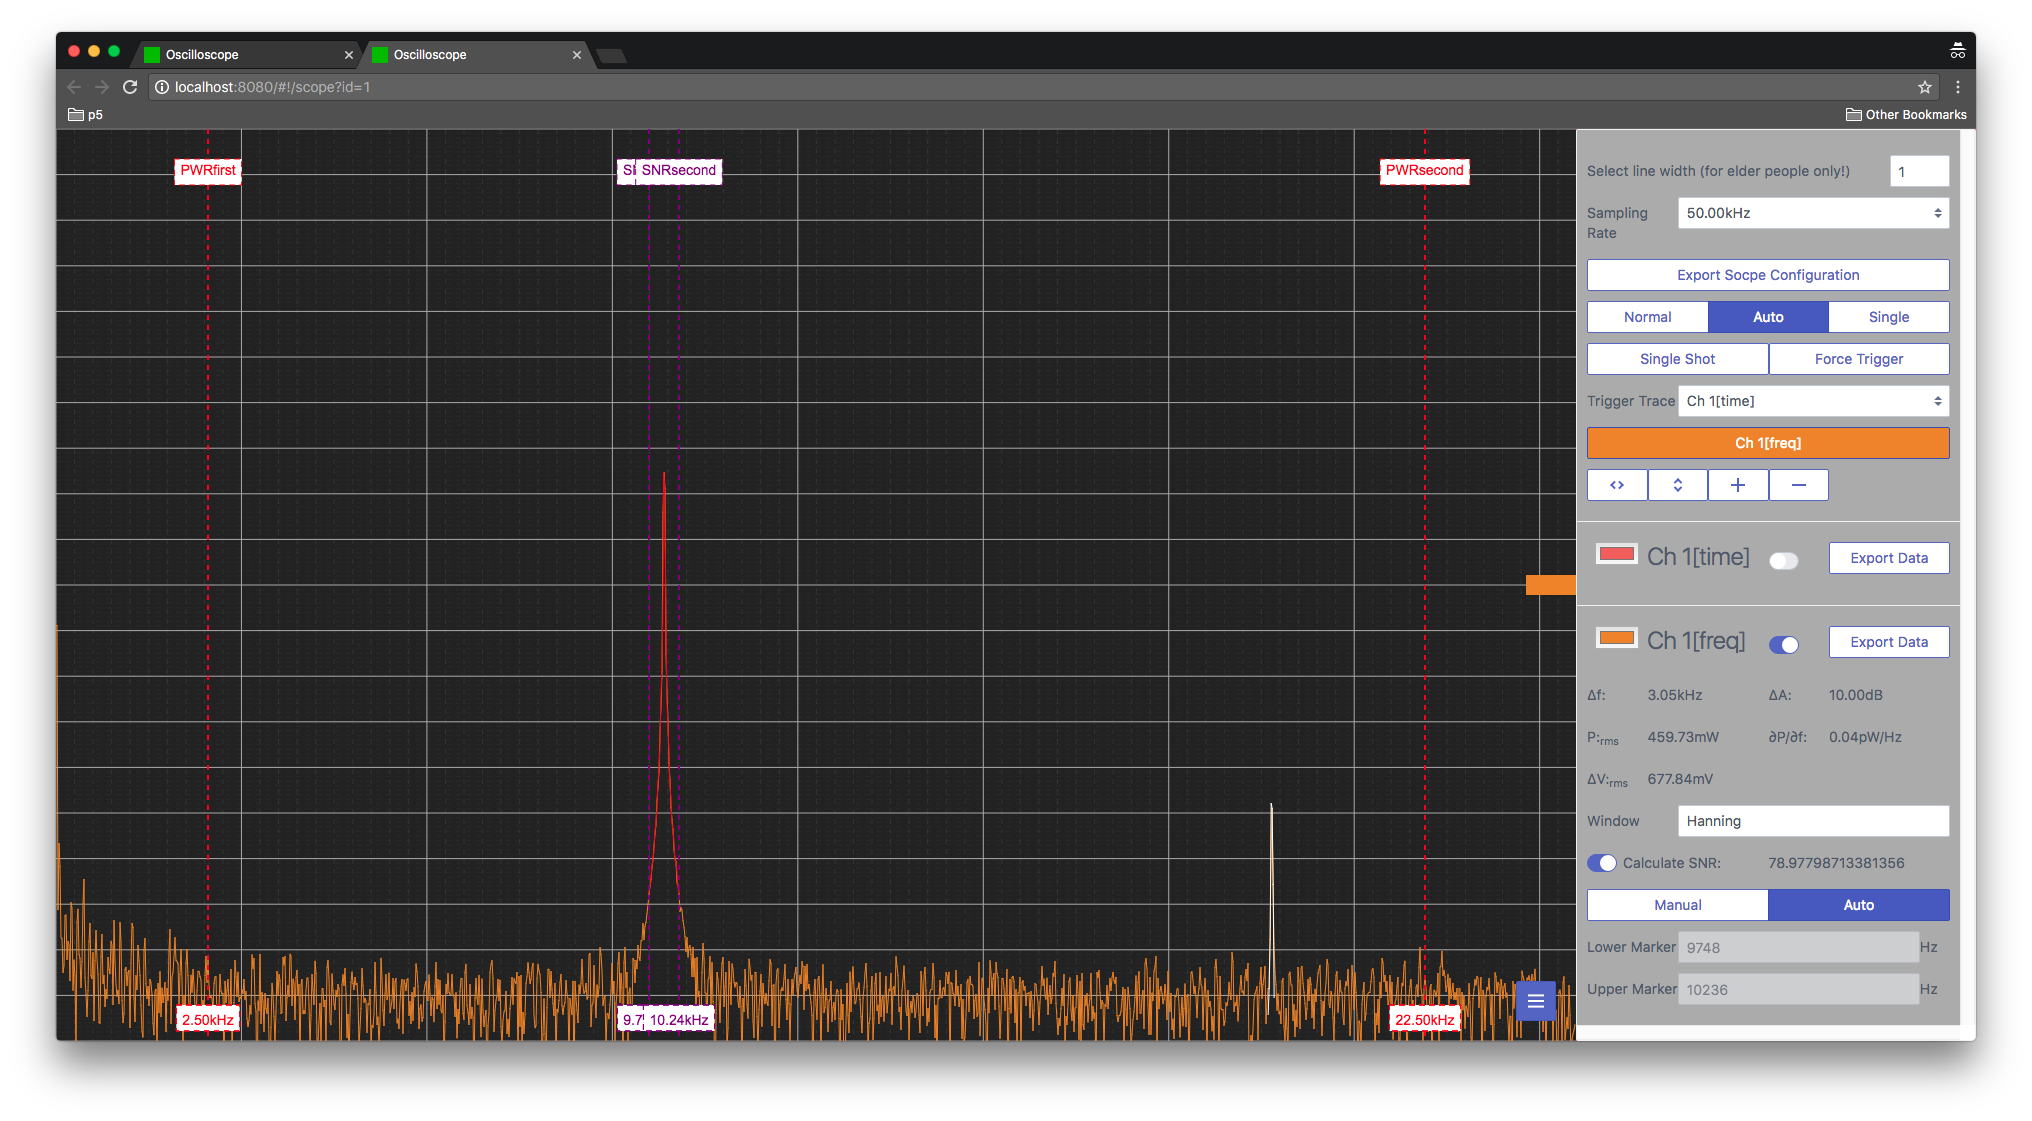
\includegraphics[width=1\textwidth]{images/scope}
\end{frame}

\begin{frame}
    \frametitle{Technologies used}

    \centering
    \begin{tikzpicture}
        \node at (0,0) {
\includegraphics[width=2cm]{images/logos/JS.jpeg}};
        \node at (4,-1) {
\includegraphics[width=2cm]{images/logos/webgl.jpeg}};
        \node at (0,-4) {
\includegraphics[width=2cm]{images/logos/uws.jpeg}};
        \node at (4,-4) {
\includegraphics[width=2cm]{images/logos/mithril.png}};
    \end{tikzpicture}
\end{frame}

\section{Results}

\begin{frame}
    \frametitle{Conclusions}
    \begin{overprint}
        \onslide<1-2>
        \centering
        \Huge\textbf{SUCCESS!}
    \end{overprint}

    \begin{overprint}
        \onslide<2>
        \centering
        \vspace{1em}
        Future Potential:
        \begin{itemize}
            \item Measurements and Analysis
            \item Optimize FPGA Resource Usage % (Filters, Features)
            \item Scope % (extend, optimize, ...)
            \item Additional Front-Ends
        \end{itemize}
    \end{overprint}
\end{frame}

% >>>


\section<handout:0| trans:0>*{Questions?} % ------------------------------- FRAME %
\end{document}
% vim: foldenable foldcolumn=4 foldmethod=marker foldmarker=<<<,>>>
